\chapter{\label{chap:results}Results and Findings}

\section{\blobdog{}}

DoG is a blob-detection technique and in this data blobs are expected to be agglomerate stellar structures among which GCs.
In Figure \ref{fig:dog-examples}, you can see that this technique finds several blobs in the different areas. The green circles indicate where blobs were found, a small/thinner circle represents a smaller blob, and a larger/fuller circle illustrates a larger blob.

A1s Figure \ref{fig:ngc5024-dog} finds only one blob, which is the globular cluster NGC 5024. In \ref{fig:palomar5-and-M5} you see a raster with a region of RA(228.0 -- 232.0) and Dec(-2.0, 2.0). Visibly present are two blobs which are both GCs. Palomar 5, which, is clearly found in the center of the raster, and M5, with its center coordinates of ($RA(229.6)$, $Dec(2.02)$) in another raster but with a large enough diameter such that its stars are also partially within the raster of Figure \ref{fig:palomar5-and-M5}. As the blob is so on and near the edge we only see half a green circle. You could see this as an indication that the raster might need to be made at a different cutoff point before running it through the next part of the pipeline. In the circumstances found in A1, where there are apart from the GCs not many stars present overall, DoG seems to work perfectly as a GC detection method. However, in areas that have a lot more stars overall, it does not only see GC's as blobs.

A2 has been rasterized and run DoG on twice, once with $\SI{4.0}{\degree}\times\SI{4.0}{\degree}$ raster parameters and once with $\SI{2.0}{\degree}\times\SI{2.0}{\degree}$ raster parameters. Figures \ref{fig:M71-dog-4b4} and \ref{fig:M71-dog-2b2} both show a variation of blobs that were found, among which the GC M71. The $\SI{2.0}{\degree}\times\SI{2.0}{\degree}$  is one fourth the size of the $\SI{4.0}{\degree}\times\SI{4.0}{\degree}$ raster making it a way smaller and easier area to look at as the number of blobs is less.

A3 is an area with an occasional extreme amount of stars in one large location, good examples of this situation are the Magellanic Clouds. DoG finds many blobs here, which is not unusual as there are many stellar objects present in these clouds. Many of the objects seem to be bright stars or galaxies. In \ref{fig:small-magellanic-cloud} there are no GCs but it is a busy area where it finds many blobs. In \ref{fig:large-magellanic-cloud} it finds an enormous amount of blobs. This raster contains four blobs (NGC 1696, NGC 1756, NGC 1786, and NGC 1795), however, it is not distinctly clear which ones in the image they could be, as so different blobs are found here as well.

A4 has two large galaxies (which can be seen in Figures~\ref{fig:andromeda} and~\ref{fig:triangulum}). The galaxies themselves as a whole are not seen as blobs, however, the large singular parts that make up these galaxies, identify as blobs. For more detail on A4 see Table~\ref{tb:identified-rasters-area4}.


\begin{figure}[H]
    \centering
    \begin{subfigure}[b]{0.32\textwidth}
        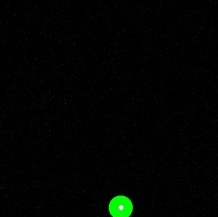
\includegraphics[width=\textwidth]{blob-dog/a1-196.0-18.0.jpg}
        \caption{\label{fig:ngc5024-dog} In A1: NGC 5024}
    \end{subfigure}
    \begin{subfigure}[b]{0.32\textwidth}
        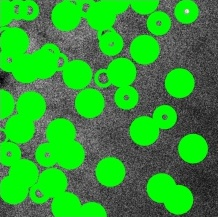
\includegraphics[width=\textwidth]{blob-dog/a2-295.0-15.0.jpg}
        \caption{\label{fig:M71-dog-4b4}In A2 (4by4): M71}
    \end{subfigure}
    \begin{subfigure}[b]{0.32\textwidth}
        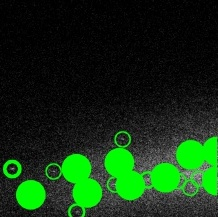
\includegraphics[width=\textwidth]{blob-dog/a3-8.0--74.0.jpg}
        \caption{\label{fig:small-magellanic-cloud}In A3: Small Magellanic Cloud}
    \end{subfigure}
    \begin{subfigure}[b]{0.32\textwidth}
        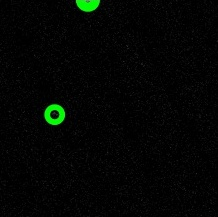
\includegraphics[width=\textwidth]{blob-dog/a1-228.0--2.0.jpg}
        \caption{\label{fig:palomar5-and-M5} In A1: Palomar 5 + M5 cutoff}
    \end{subfigure}
    \begin{subfigure}[b]{0.32\textwidth}
        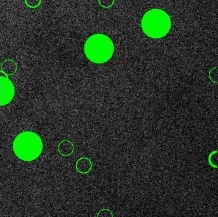
\includegraphics[width=\textwidth]{blob-dog/a2-297.0-17.0.jpg}
        \caption{\label{fig:M71-dog-2b2}In A2 (2by2): M71}
    \end{subfigure}
    \begin{subfigure}[b]{0.32\textwidth}
        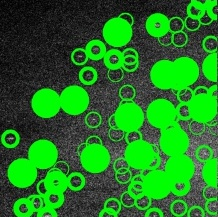
\includegraphics[width=\textwidth]{blob-dog/a3-72.0--70.0.jpg}
        \caption{\label{fig:large-magellanic-cloud}In A3: Large Magellanic Cloud}
    \end{subfigure}
    \begin{subfigure}[b]{0.32\textwidth}
        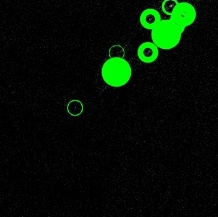
\includegraphics[width=\textwidth]{blob-dog/a4-8.0-38.0.jpg}
        \caption{\label{fig:andromeda}In A4: Andromeda Galaxy}
    \end{subfigure}
    \begin{subfigure}[b]{0.32\textwidth}
        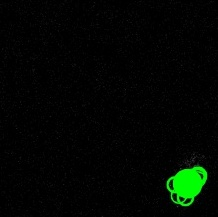
\includegraphics[width=\textwidth]{blob-dog/a4-20.0-30.0.jpg}
        \caption{\label{fig:triangulum}In A4: Triangulum Galaxy}
    \end{subfigure}

    \caption{\label{fig:dog-examples} Interesting examples of the blobs found by DoG}
\end{figure}



\subsection{Remaining Rasters}
The \blobdog{} filter was run across all the rasters of the area with varying
thresholds. The number of remaining rasters depend on the threshold that was set
regarding the intensity of the blob-detection on the data in the raster. In
Table~\ref{tb:number-of-remaining-rasters} the number of remaining rasters, from each area, are shown for the different thresholds.

\begin{table}[H]
    \centering
    \caption{Rasters remaining after the execution of \blobdog{} at Varying Thresholds}
    \label{tb:number-of-remaining-rasters}
    \begin{tabular}{l c c c}
        \toprule
        Area          & Threshold = $0.5$ & Threshold = $0.2$ & Total Number of Rasters \\
        \midrule
        Area 1        & 7                 & 8                 & 512                     \\
        Area 2 (4by4) & 7                 & 9                 & 12                      \\
        Area 2 (2by2) & 16                & 28                & 35                      \\
        Area 3        & 23                & 39                & 285                     \\
        Area 4        & 19                & 60                & 120                     \\
        \bottomrule
    \end{tabular}
\end{table}

% The raster size is \tx{ra_step} x \tx{dec_step} = 4 x 4. except for area 2 as this are is quite dense ans also smaller, it is instead a 2 x 2.
When you set the threshold too low you will detect one or more blobs in every raster. For A1 the threshold was set to 0.1 and it found blobs in all 512 rasters. Then the intensity of the detection is too high, and so single stars are detected as blobs.

\subsection{A1, A2, and A3 - Filtering Rasters with Known GCs}

%\TODO{fix $RA_{start}$, $Dec_{start}$}
\textbf{A1} has 7 out of 12 known GCs detected within a threshold of 0.2. Additionally, it detects blobs in another raster that does not contain a known GC. This raster is in the region with a starting RA and Dec (RA-start, Dec-start) of (152.0, 10.0) and a range of $\SI{4.0}{\degree}\times\SI{4.0}{\degree}$,  where it finds a blob at approximately $RA$: $152\si{\degree}$ and $Dec$:
$12\si{\degree}$ at this position there is a dwarf galaxy.
When searching between the thresholds of 0.2 and 0.1, we find that: In the case that the threshold=.15 it mostly does find the known GCs. The known GCs that are only detected then are for example: Koposov 1 which is a low-luminosity globular cluster~\cite{Koposov2007}, Palomar 3 which is one of the most distant GCs~\cite{Sharina2018} with a magnitude of 14.26 and a distance of $\sim$96 kpc, and Palomar 4 which has an even larger magnitude of 15.65 and distance of $\sim$109 kpc~\cite{listGC} .
% Willman 1 should have been detected with a magnitude of $\sim$ -2 and a distance of $\sim$38 kpc~\cite{Willman2011} but it wasn't
They are not detected by \blobdog{} because the size of the blob/cluster in these cases is quite small as they are located farther away or are of lower luminosity.

\textbf{A2} has two similar outputs for the different types of rasterization bounds. They both detect the one GC present in thais area.
A2 (4x4) detects blobs in 7 rasters with a threshold of 0.5 and 9 rasters with a threshold of 0.2.
A2 (2x2) finds that in 16 rasters one or more blobs get detected when the threshold is set to 0.5 and 28 rasters remain at a threshold of 0.2. The raster in which this blob should be visible, has the region RA(297.0, 299.0), Dec(17.0,19.0)), and is present among the remaining rasters under threshold 0.5. A2 (2x2) is rastered into 35 windows, which is a much smaller amount than A1. However, the number of stars per raster is higher and the area that is split up in these files is smaller, so what you see in the image is a denser appearance of the stars.\\

\textbf{A3} detects blobs in 39 out of 285 rasters with a threshold set to 0.2. At a threshold of 0.5 it will find one or more blobs in 23 rasters. And all rasters of the known GCs, but one (Arp Madore 1), have blobs detected under a threshold of 0.2. It is understandable that Arp Madore 1 does not get detected as a blob because it is one of most distant known GCs of the Milky Way \cite{Arp-Madore-1}.

The precise GCs that were found can be seen in the overview in Table~\ref{tb:areas-found-rasters-0.2}.

% \TODO{fix this table, possibly add one word as a description of the GC (distant, small, large, close, normal)}

\begin{table}[H]
    \centering
    \caption{What known GCs are getting detected for a threshold of 0.2}
    \label{tb:areas-found-rasters-0.2}
    \begin{tabular}{lL{0.2\linewidth}lL{0.2\linewidth}lL{0.2\linewidth}}
        \toprule
        GC        & \blobdog{}s Present GCs & GC     & \blobdog{}s Present GCs & GC           & DoGs Present GCs \\
        \midrule
        Area 1    &                         & Area 2 &                         & Area 3       &                  \\
        \midrule
        M3        & Present                 & M71    & Present                 & 47 Tucanae   & Present          \\
        M5        & Present                 &        &                         & NGC 121      & Present          \\
        NGC 5024  & Present                 &        &                         & NGC 1049     & Present          \\
        NGC 4147  & Present                 &        &                         & NGC 362      & Present          \\
        NGC 5053  & Present                 &        &                         & NGC 1261     & Present          \\
        NGC 5466  & Present                 &        &                         & NGC 1466     & Present          \\
        Koposov 1 &                         &        &                         & NGC 1629     & Present          \\
        Palomar 3 &                         &        &                         & NGC 1644     & Present          \\
        Palomar 4 &                         &        &                         & NGC 1651     & Present          \\
        Palomar 5 & Present                 &        &                         & NGC 1652     & Present          \\
        GCI 38    &                         &        &                         & NGC 1696     & Present          \\
        Willman 1 &                         &        &                         & NGC 1756     & Present          \\
                  &                         &        &                         & NGC 1783     & Present          \\
                  &                         &        &                         & NGC 1786     & Present          \\
                  &                         &        &                         & NGC 1795     & Present          \\
                  &                         &        &                         & NGC 1841     & Present          \\
                  &                         &        &                         & Arp Madore 1 &                  \\
        \bottomrule
    \end{tabular}
\end{table}








\subsection{A4 - Finding Other Stellar Structures}

\textbf{A4} does not contain any known GCs but has 60 out of 120 raster files containing blobs according to DoG using a threshold value of 0.2. And 19 at a threshold of 0.5. Some of the stellar structures are described in Table~\ref{tb:identified-rasters-area4}.


\begin{table}[H]
    \centering
    \caption{Some Identifiable Rasters found Area 4}
    \label{tb:identified-rasters-area4}
    \begin{tabular}{L{0.2\textwidth}L{0.3\textwidth}L{0.4\textwidth}}
        \toprule
        \textbf{coordinates in \tx{ra} - \tx{dec}} & \textbf{Identified As}                                                                                             & \textbf{Blob Description}                                                                                                                                            \\
        \midrule
        \tx{10.0 - 41.0}                           & Andromeda                                                                                                          & Massive stars and the dwarf galaxy NGC 205 within Andromeda are seen as blobs but Andromeda itself is not, probably because of the shape.                            \\
        \tx{23.4 - 30.0}                           & Triangulum Galaxy M33                                                                                              & Massive circular shape is detected which is circled by more subtle blobs. The main shape is the spiral galaxy.                                                       \\
        \tx{(0 to 4)-(62 to 66)}                   & Supernova Remnant SNR G116.9+00.1,  open star cluster st 18 within the Little Rosette Nebula, dark nebula LDN 1268 & The raster is quite busy, it contains a super nova remnant, an open star cluster, a dark nebula and many stars. Ten large blobs and seven smaller ones are detected. \\
        \bottomrule
    \end{tabular}
\end{table}

\subsection{Rasters Graph Comparing DoG Findings to Respective Areas}

Figure~\ref{fig:filtered-dog-rasters} shows rasters containing blobs as identified by dog across the four areas. All four areas are represented as a plot of rasters indicating where DoG finds \textit{known GCs}, \textit{other blobs}, and \textit{no blobs}. It also shows what rasters should have found GCs but instead have it be the \textit{missing known GCs} locations. To give a clear idea of where you can picture these locations, it is displayed below the scatter-plot of stars.
\TODO{The 4x4 raster plot has wrong naming for the Axes }
\begin{figure}[H]
    \centering

    \begin{subfigure}[b]{0.49\textwidth}
        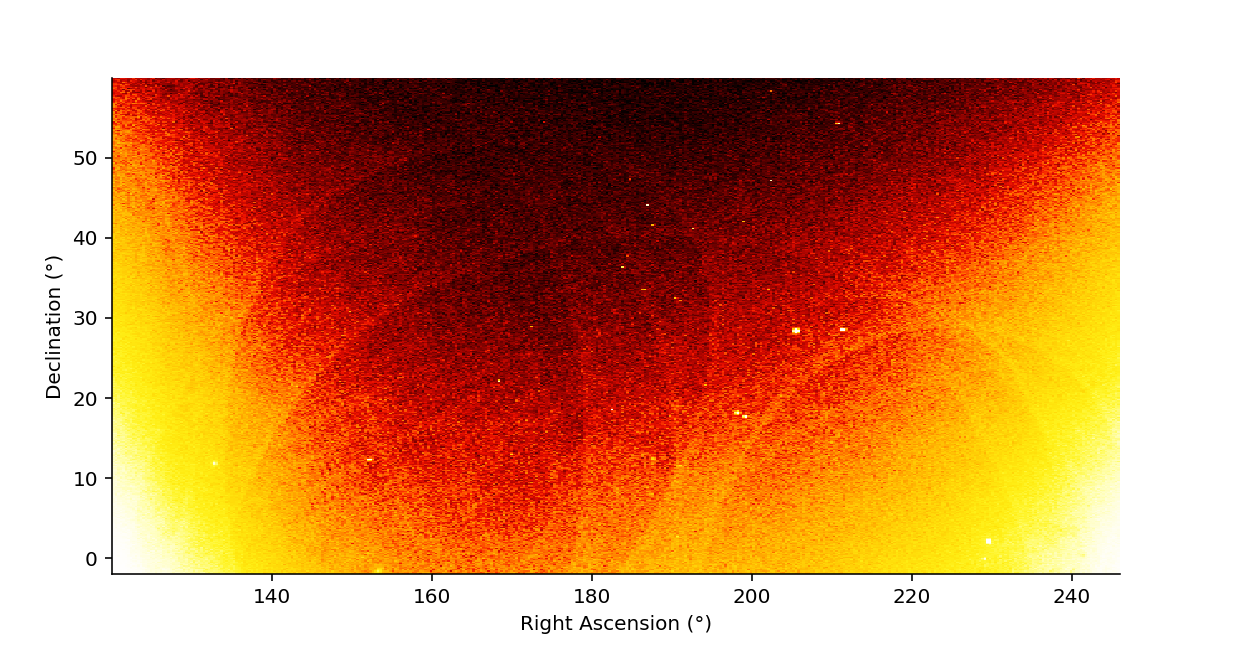
\includegraphics[height=0.6\textwidth]{scatterplots/area1-scatterplot.png}
        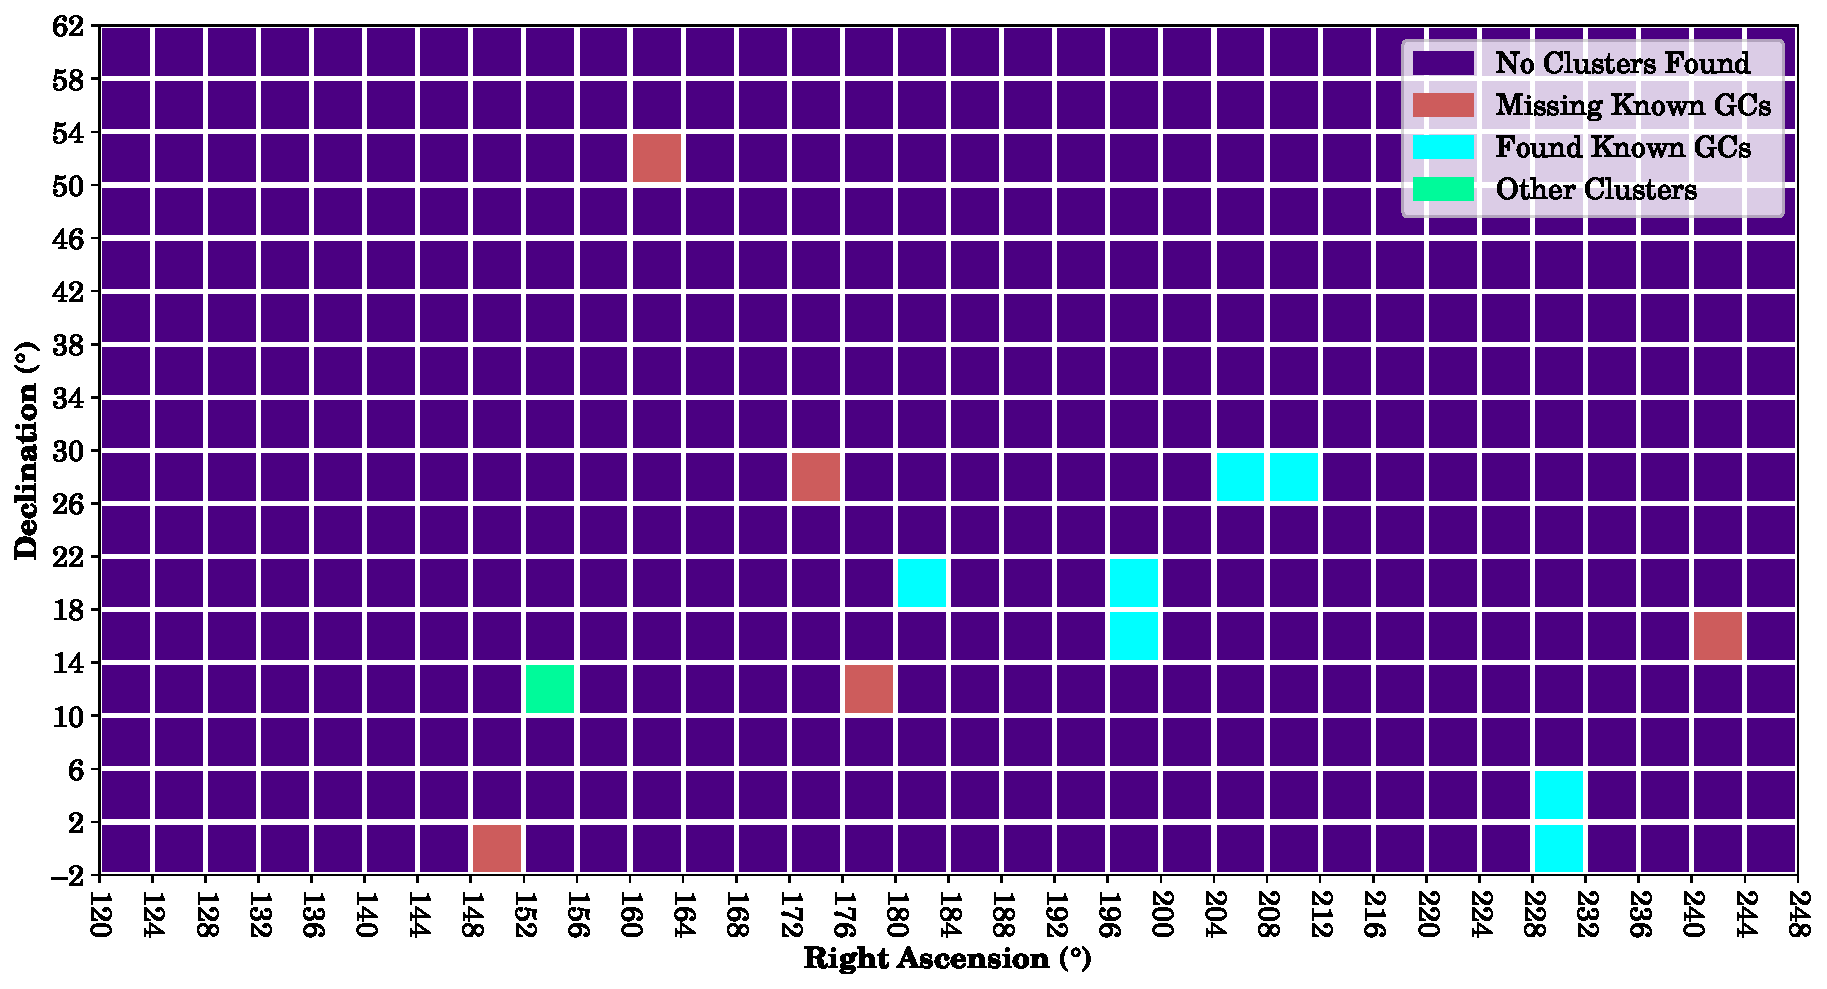
\includegraphics[height=0.6\textwidth]{./figures/rasters/grids/grid-dog-a1.pdf}
        \caption{A1}
        \label{fig:a1-dog-overview}
    \end{subfigure}
    \begin{subfigure}[b]{0.49\textwidth}
        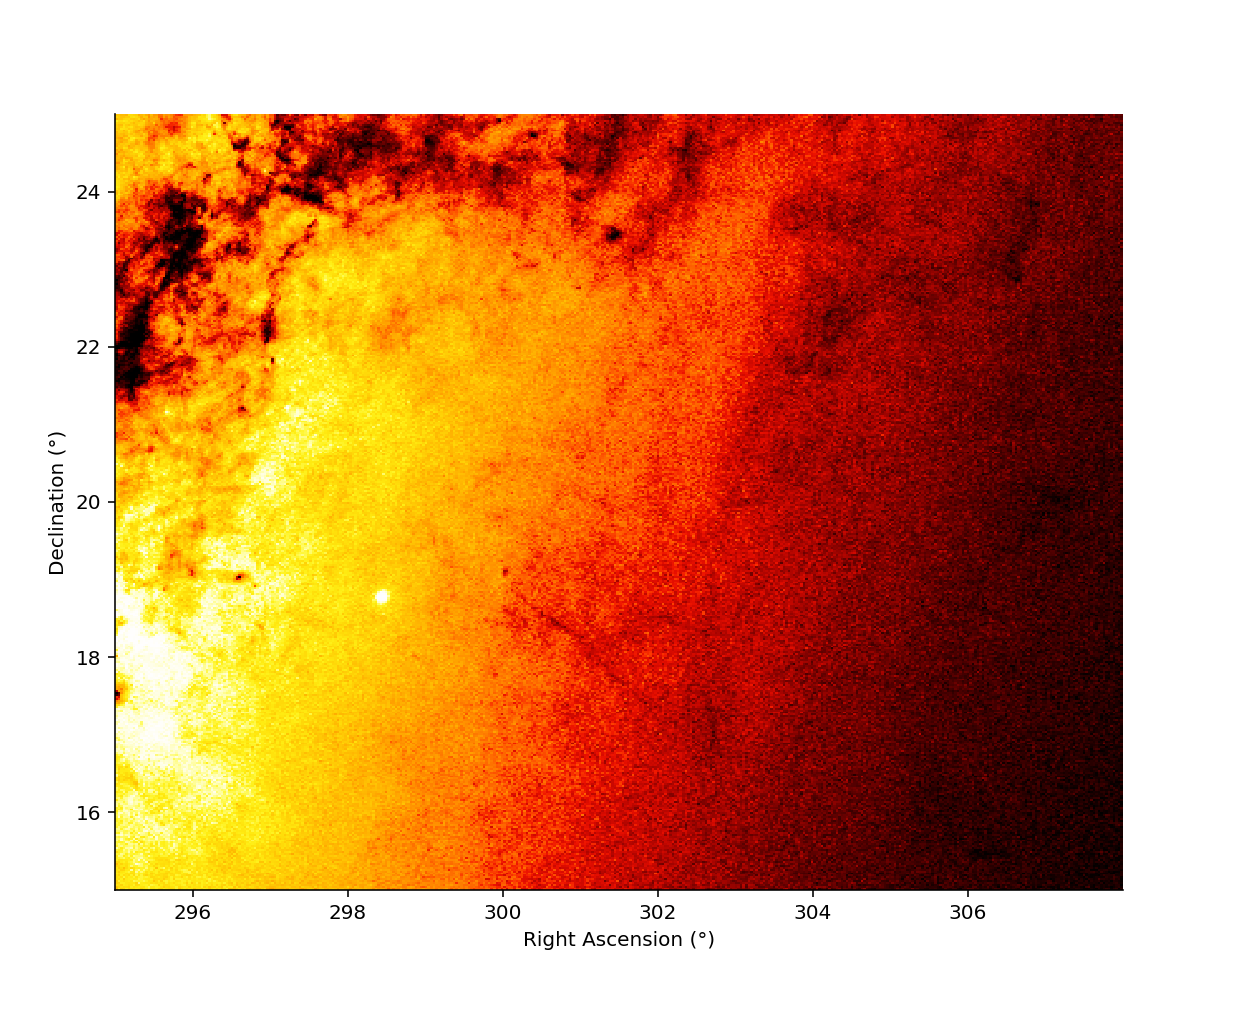
\includegraphics[height=0.6\textwidth]{scatterplots/area2-scatterplot.png}
        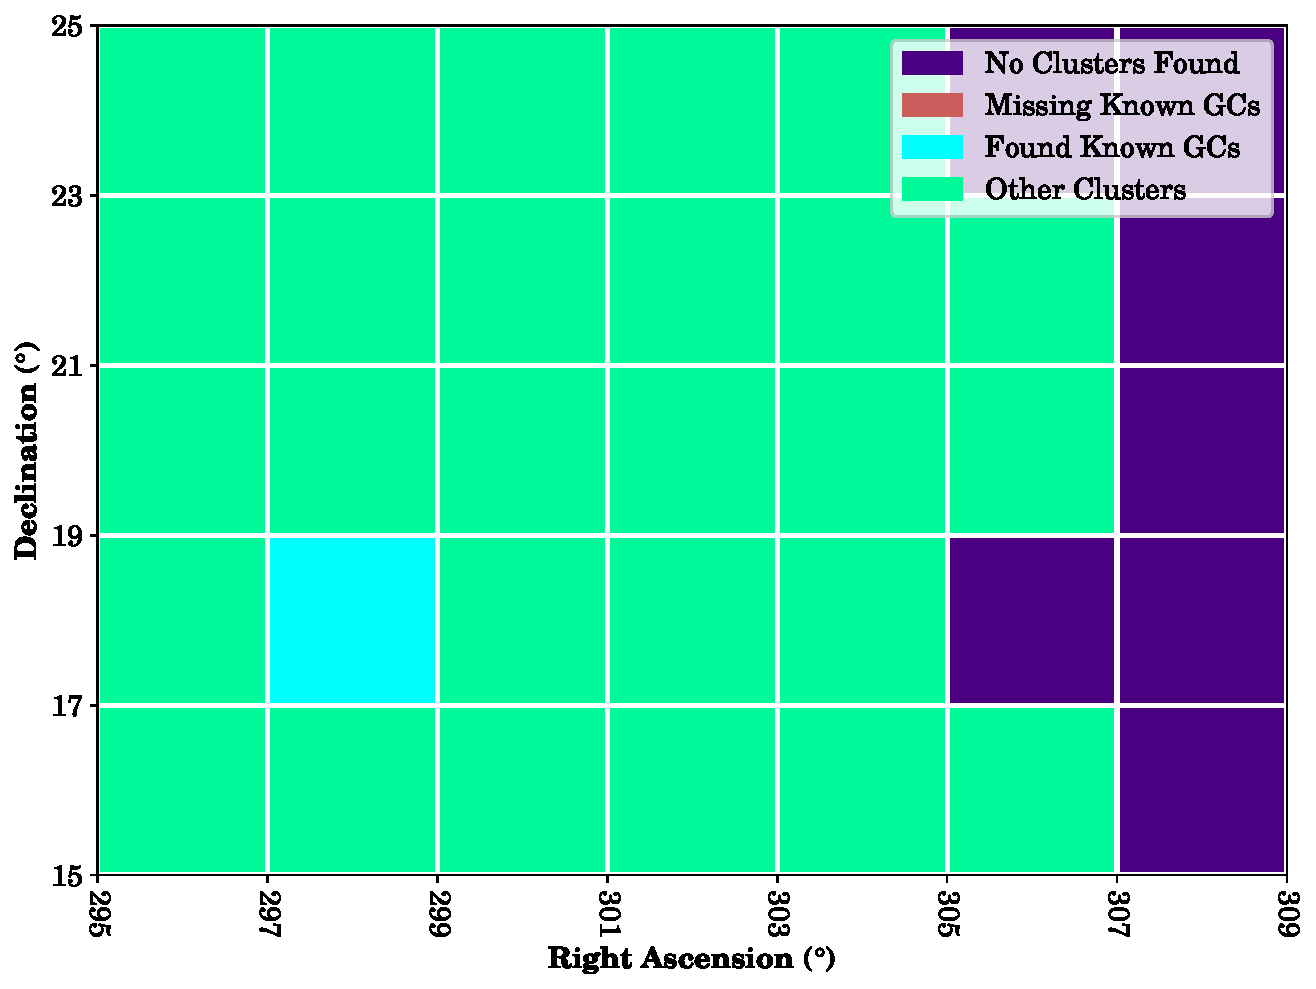
\includegraphics[height=0.6\textwidth]{./figures/rasters/grids/grid-dog-a2.pdf}
        \caption{A2}
        \label{fig:a2-dog-overview}
    \end{subfigure}

    \begin{subfigure}[b]{0.49\textwidth}
        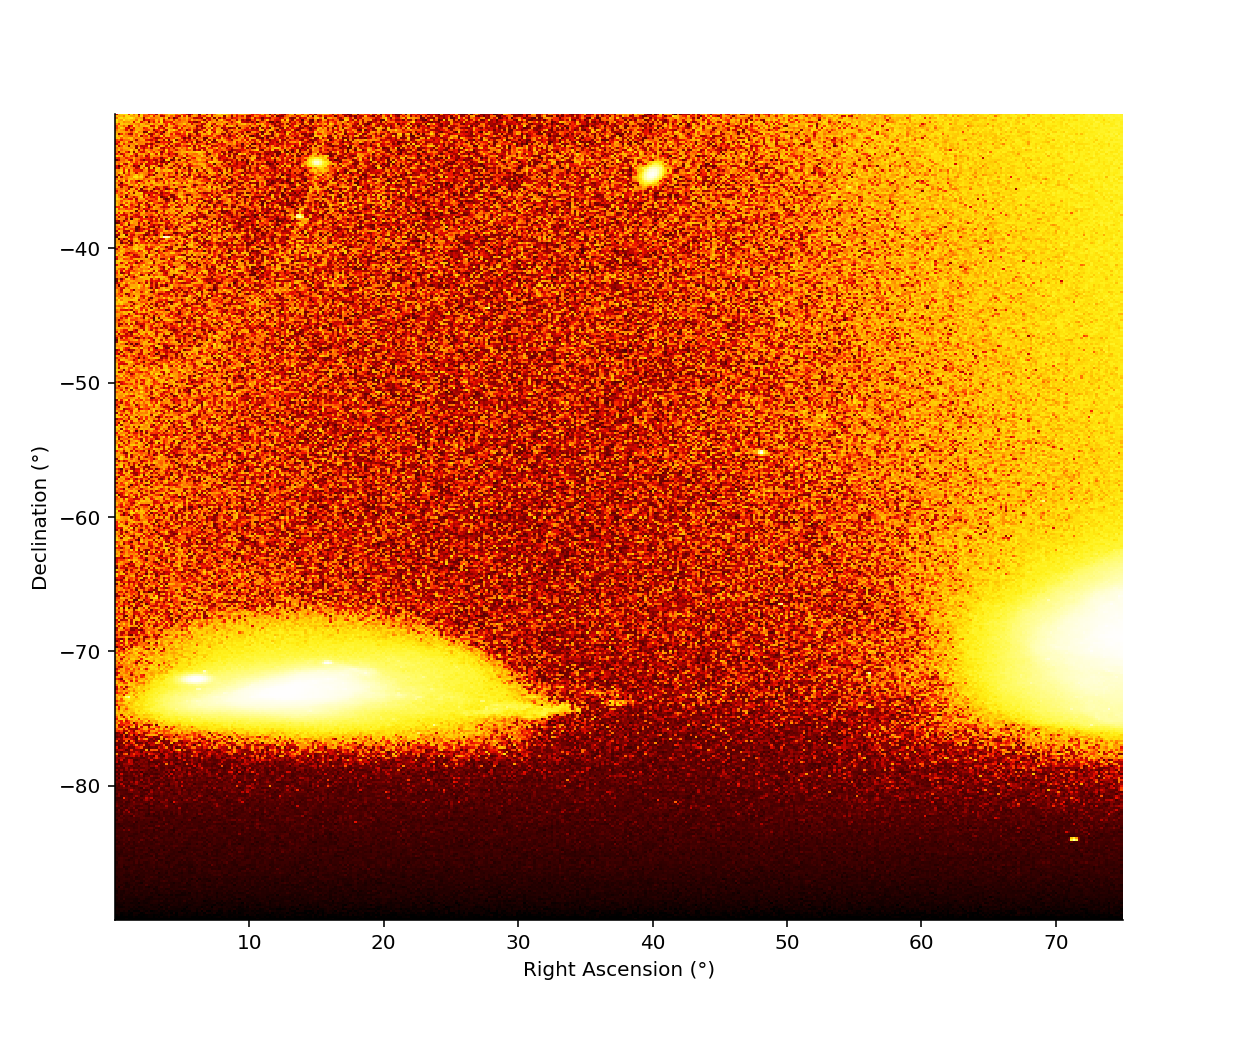
\includegraphics[ height=0.6\textwidth]{scatterplots/area3-scatterplot.png}
        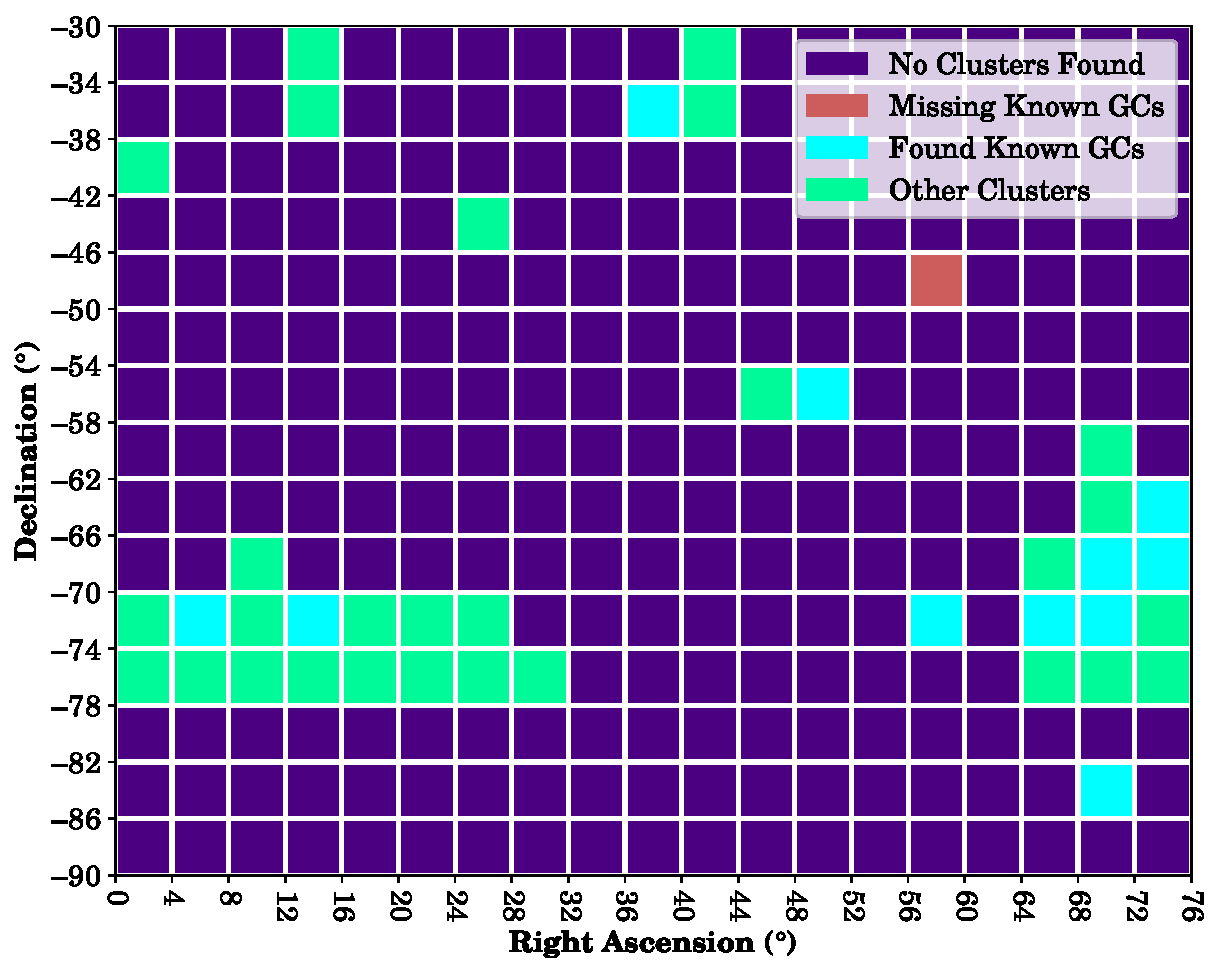
\includegraphics[height=0.6\textwidth]{./figures/rasters/grids/grid-dog-a3.pdf}
        \caption{A3}
        \label{fig:a3-dog-overview}
    \end{subfigure}
    \begin{subfigure}[b]{0.49\textwidth}
        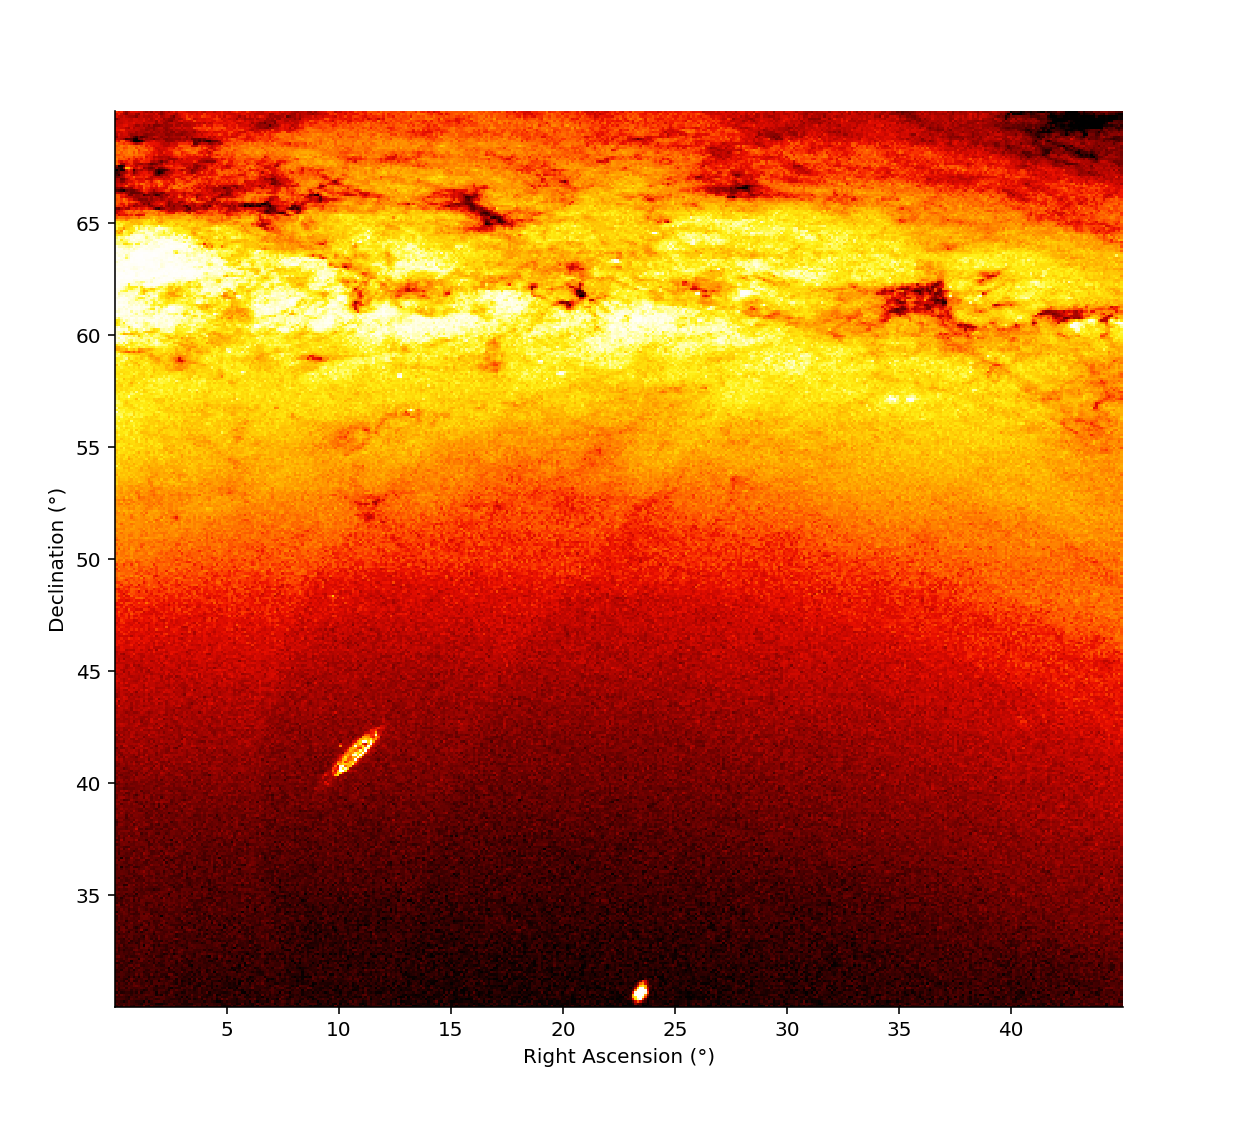
\includegraphics[ height=0.6\textwidth]{scatterplots/area4-scatterplot.png}
        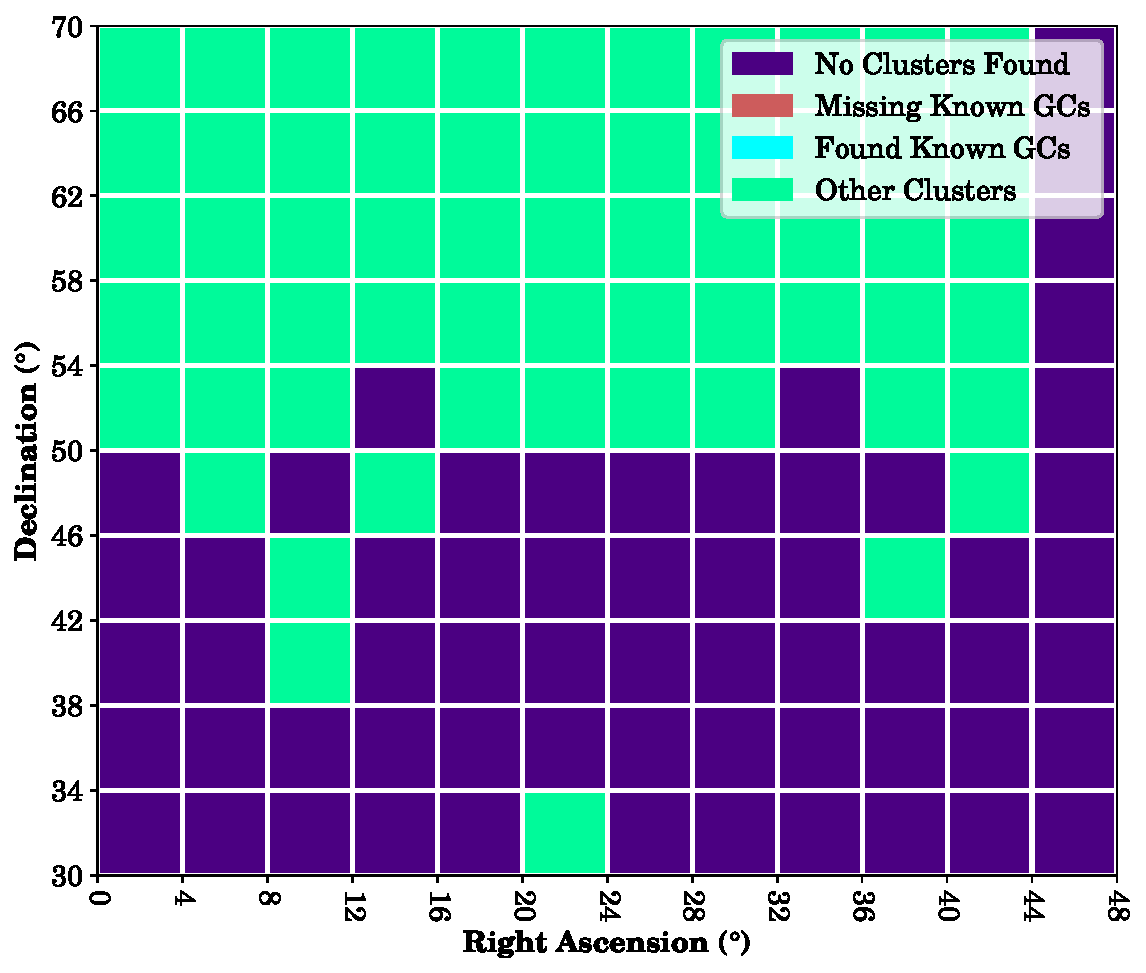
\includegraphics[height=0.6\textwidth]{./figures/rasters/grids/grid-dog-a4.pdf}
        \caption{A4}
        \label{fig:a4-dog-overview}
    \end{subfigure}

    \caption{Rasters-and scatter-plot comparison where DoG was run with threshold set to 0.2}
    \label{fig:filtered-dog-rasters}
\end{figure}

This Figure makes clear that areas that have a high number of stars  or a high contrast in star density (i.e. A1, A2, and A3) has many blobs detected by DoG. From the A2 and A4 raster figure to scatter-plot comparison we see that it finds blobs at the yellow bright parts of the scatter-plots. A3 has blobs detected at the locations of the Magellanic Clouds. We can also see that ate the blacker dark regions in the scatter-plots represented in the raster graph, there are near to no blobs found. The scatter-plot of A1 has the yellow brightest parts in the corners, however, in comparison to the number of stars present in the brightest parts of the other areas it contains less stars.(plot might not be representative in comparison to other areas scatter-plots)

\newpage

\section{Ant}


To understand how this Algorithm looks like in different types of regions, we take a closer look at some example areas in the Figures of \ref{fig:scatterplot-heatmaps-A12} and \ref{fig:scatterplot-heatmaps-A34}. These figures are an indication of the Ant Colony algorithm functioning as they are intended, zoning in on star clusters through appointed pheromone values to stars in dense areas. There is a comparison of the densities of stars in different raster areas and how the Ant Colony algorithm handles them is visualized in the heat-maps depicted below the scatter-plots of the stars in the rasters.

Both Figure~\ref{fig:heat-ngc4147} and Figure~\ref{fig:heat-palomar5} representing A1, have yellow spots depicting stars with high pheromone values. In these rasters you can see relatively clearly that the Ant Colony algorithm marks the locations of the GCs with higher pheromone values.

A2 (2by2) is a more zoomed in version of the (4by4) raster that focuses on the present GC of this area. The heat-maps of both Figure~\ref{fig:heat-M71-dog-4b4} and Figure~\ref{fig:heat-M71-dog-2by2} are very dark. Figure~\ref{fig:heat-M71-dog-2by2} shows some small and nearly invisible pheromone spots and has a slightly higher maximum pheromones of \num{0.75} than the Figure~\ref{fig:heat-M71-dog-4b4} of (4by4) with a maximum pheromone of \num{0.55}. \textbf{As the (2by2) raster gets a better result here we will mainly be looking at the (2by2) raster information from now on.}

A3 showing its two Magellanic Clouds has a similar occurrence of an incredibly dense stellar region that does not get represented well in the pheromone heat-map, showing (in black) how the Ant Colony algorithm is handling these type of areas. Table~\ref{tb:pheromone-mean-areas} displays the number of stars ($N_{\text{stars}}$) for each sub-figure in Figure~\ref{fig:scatterplot-heatmaps-A12} and Figure~\ref{fig:scatterplot-heatmaps-A34}, showing that the $N_{\text{stars}}$ of A2 and A3 are more than a two-hundred-thousand and even go up to a million stars, and the rasters shown of A1 and A4 are less than thirty-thousand. This difference is huge and would explain the behavior of the Ant Colony algorithm depicted in the heat-maps that for A3 are incredibly dark.

A4 has two examples of the algorithms effect on huge Galaxies. The Galaxies locations in the heat-maps are depicted as more dense red smudges, that are noticeable but not the brightest areas in the heat-maps. The highest pheromone values emerge in a cluster of stars that occurs for an unknown reason. This might be a group of stars worth looking into and worth further investigating with the third part of this pipeline (\ref{sec:data-clustering})

\TODO{redo the plotting of the heatmaps}
\TODO{possibly change  the choice of plots and maybe chose less plots}


\begin{figure}[H]
    \centering
    \begin{subfigure}[b]{0.24\textwidth}
        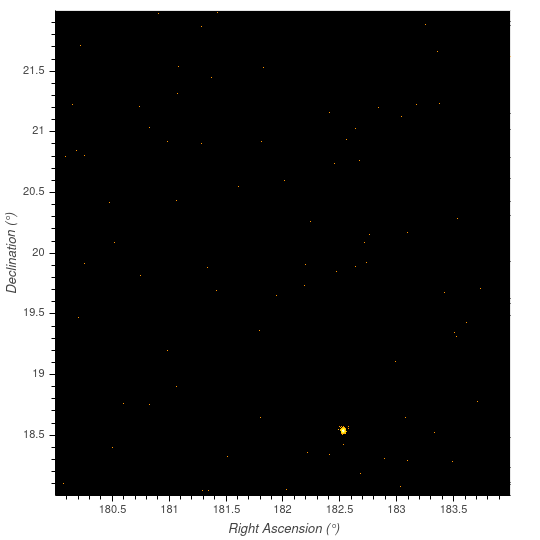
\includegraphics[width=\textwidth]{heatmaps/scatter-a1-180.0-18.0-ngc4147.png}
        \caption{\label{fig:scatter-ngc4147} A1: NGC 4147}
    \end{subfigure}
    \begin{subfigure}[b]{0.24\textwidth}
        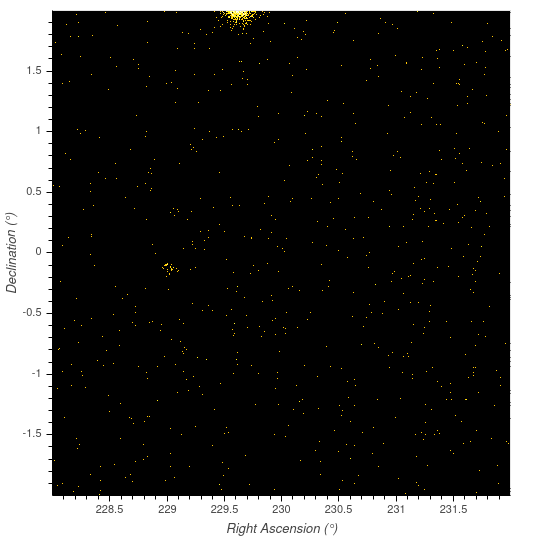
\includegraphics[width=\textwidth]{heatmaps/scatter-a1-palomar5+m5.png}
        \caption{\label{fig:scatter-palomar5} A1: Palomar 5}
    \end{subfigure}
    \begin{subfigure}[b]{0.24\textwidth}
        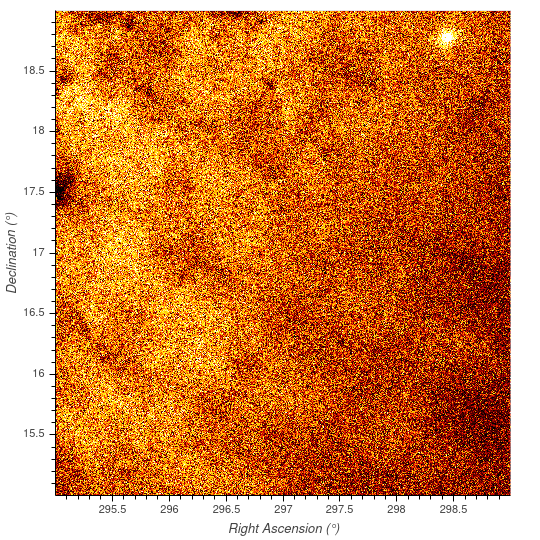
\includegraphics[width=\textwidth]{heatmaps/scatter-a2-gc-4x4.png}
        \caption{\label{fig:scatter-M71-dog-4b4}A2 (4by4): M71}
    \end{subfigure}
    \begin{subfigure}[b]{0.24\textwidth}
        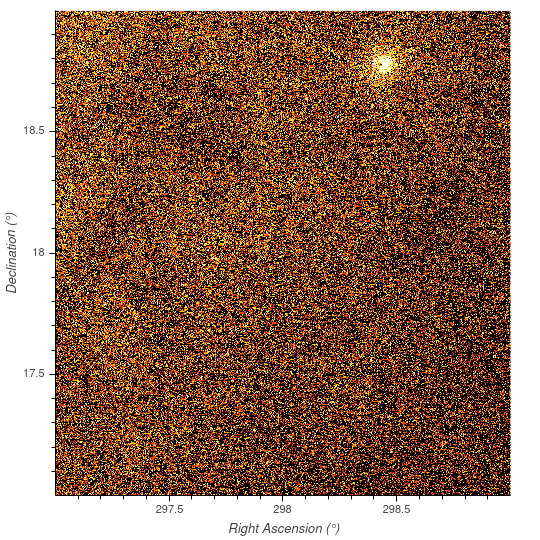
\includegraphics[width=\textwidth]{heatmaps/scatter-a2-gc-2x2.png}
        \caption{\label{fig:scatter-M71-dog-2b2}A2 (2by2): M71}
    \end{subfigure}
    \begin{subfigure}[b]{0.24\textwidth}
        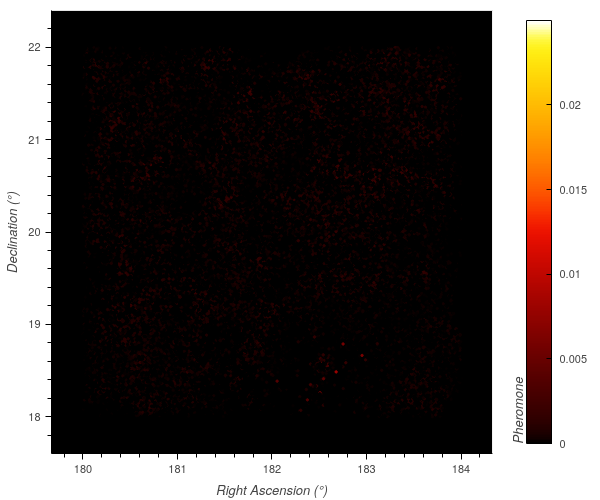
\includegraphics[width=\textwidth]{heatmaps/pheromone-heatmap-a1-180.0-18.0.png}
        \caption{\label{fig:heat-ngc4147} A1: NGC 4147}
    \end{subfigure}
    \begin{subfigure}[b]{0.24\textwidth}
        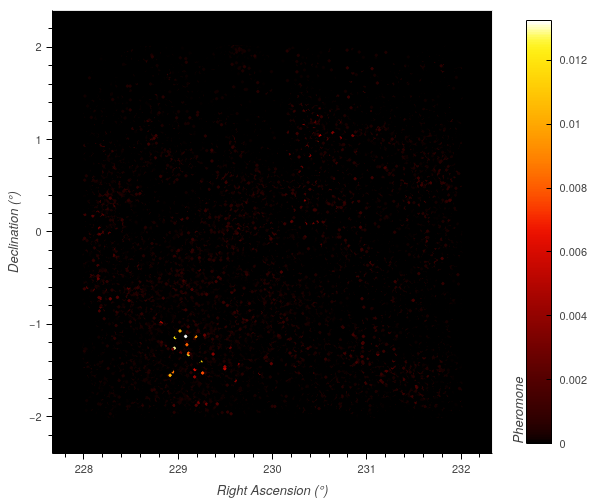
\includegraphics[width=\textwidth]{heatmaps/pheromone-heatmap-a1-228.0--2.0.png}
        \caption{\label{fig:heat-palomar5} A1: Palomar 5}
    \end{subfigure}
    \begin{subfigure}[b]{0.24\textwidth}
        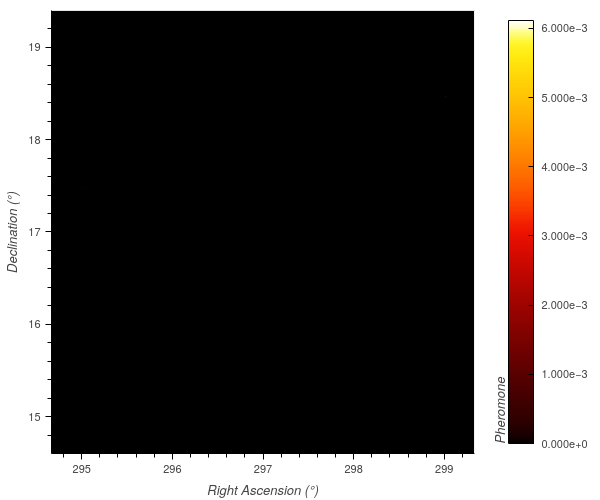
\includegraphics[width=\textwidth]{heatmaps/pheromone-heatmap-a2-295.0-15.0.png}
        \caption{\label{fig:heat-M71-dog-4b4}A2 (4by4): M71}
    \end{subfigure}
    \begin{subfigure}[b]{0.24\textwidth}
        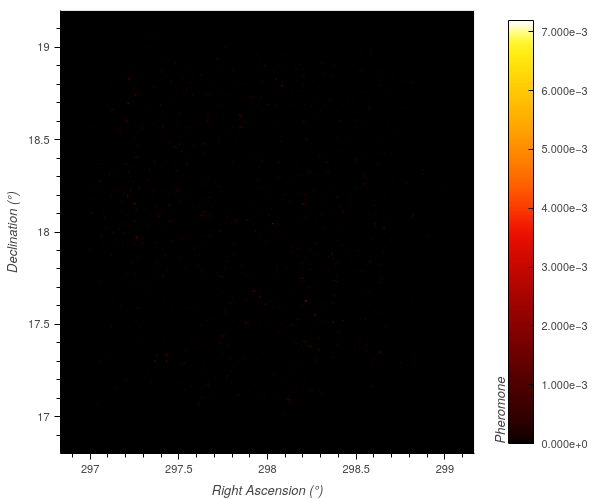
\includegraphics[width=\textwidth]{heatmaps/pheromone-heatmap-a2-297.0-17.0.png}
        \caption{\label{fig:heat-M71-dog-2by2}A2 (2by2): M71}
    \end{subfigure}
    \caption{\label{fig:scatterplot-heatmaps-A12} Scatterplots (top) vs. Heat-maps (below) of varying rasters of A1 and A2}
\end{figure}



\begin{figure}[H]
    \centering
    \begin{subfigure}[b]{0.24\textwidth}
        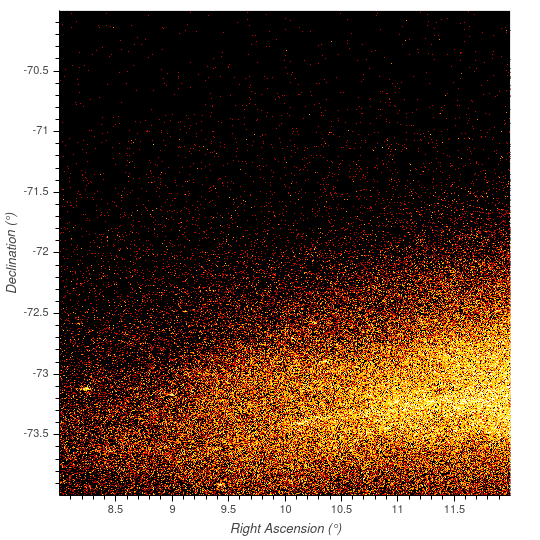
\includegraphics[width=\textwidth]{heatmaps/scatter-a3-gc-small-MC.png}
        \caption{\label{fig:scatter-small-magellanic-cloud}A3: Small Magellanic Cloud}
    \end{subfigure}
    \begin{subfigure}[b]{0.24\textwidth}
        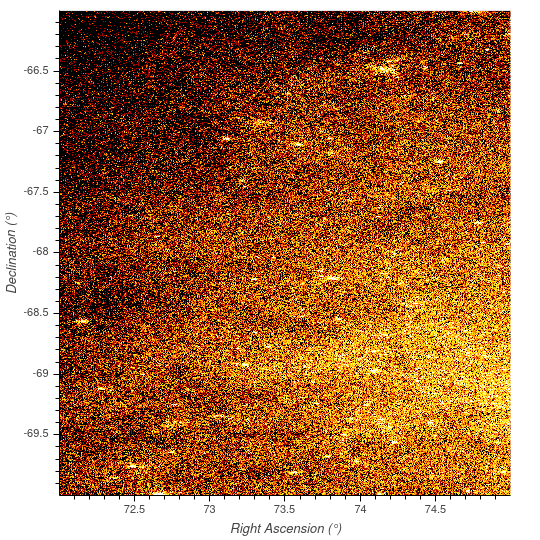
\includegraphics[width=\textwidth]{heatmaps/scatter-a3-gc-large-MC.png}
        \caption{\label{fig:scatter-large-magellanic-cloud}A3: Large Magellanic Cloud}
    \end{subfigure}
    \begin{subfigure}[b]{0.24\textwidth}
        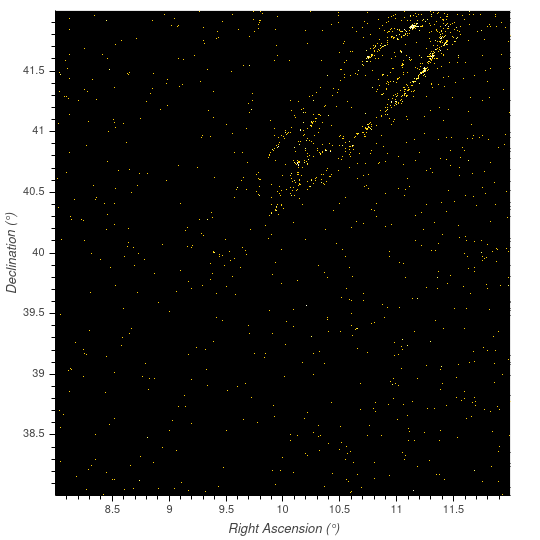
\includegraphics[width=\textwidth]{heatmaps/scatter-a4-andromeda.png}
        \caption{\label{fig:scatter-andromeda}A4: Andromeda Gal}
    \end{subfigure}
    \begin{subfigure}[b]{0.24\textwidth}
        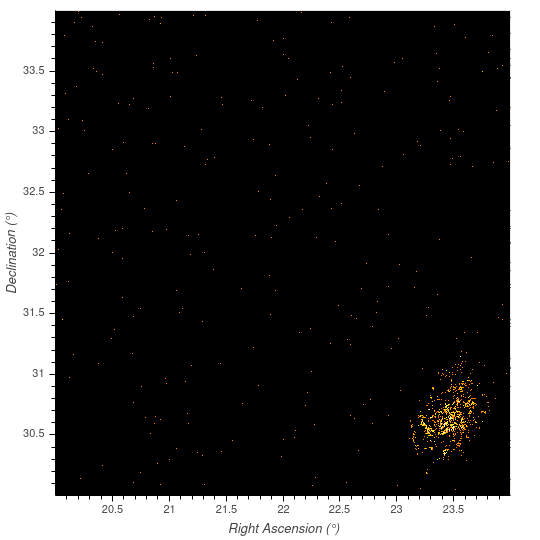
\includegraphics[width=\textwidth]{heatmaps/scatter-a4-triangulum.png}
        \caption{\label{fig:scatter-triangulum}A4: Triangulum Gal}
    \end{subfigure}
    \begin{subfigure}[b]{0.24\textwidth}
        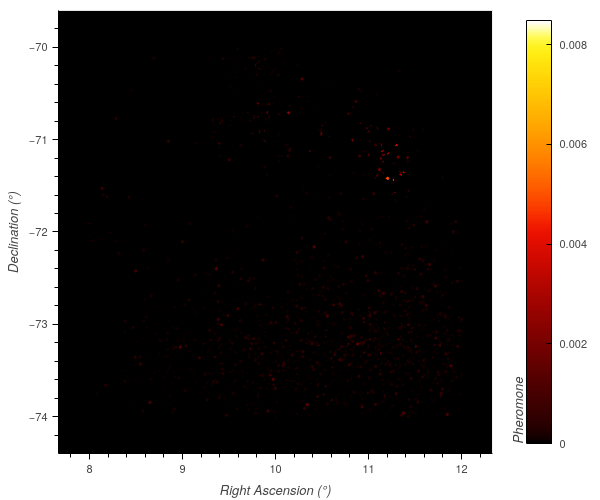
\includegraphics[width=\textwidth]{heatmaps/pheromone-heatmap-a3-8.0--74.0.png}
        \caption{\label{fig:heat-small-magellanic-cloud}A3: Small Magellanic Cloud}
    \end{subfigure}
    \begin{subfigure}[b]{0.24\textwidth}
        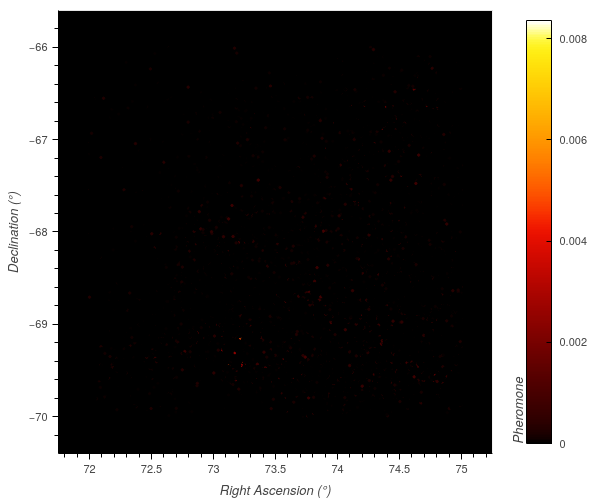
\includegraphics[width=\textwidth]{heatmaps/pheromone-heatmap-a3-72.0--70.0.png}
        \caption{\label{fig:heat-large-magellanic-cloud}A3: Large Magellanic Cloud}
    \end{subfigure}
    \begin{subfigure}[b]{0.24\textwidth}
        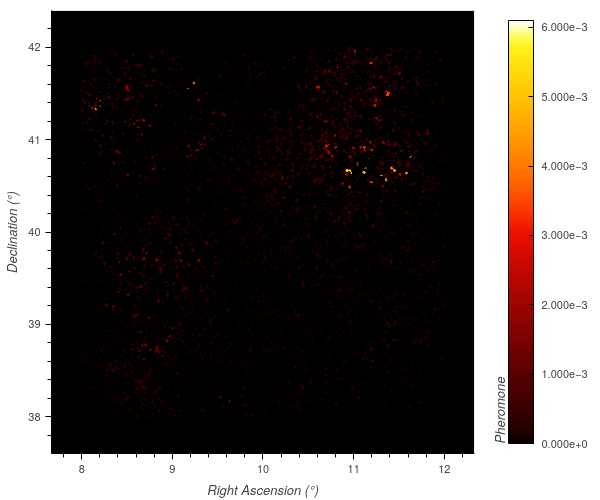
\includegraphics[width=\textwidth]{heatmaps/pheromone-heatmap-a4-8.0-38.0.png}
        \caption{\label{fig:heat-andromeda}A4: Andromeda Gal}
    \end{subfigure}
    \begin{subfigure}[b]{0.24\textwidth}
        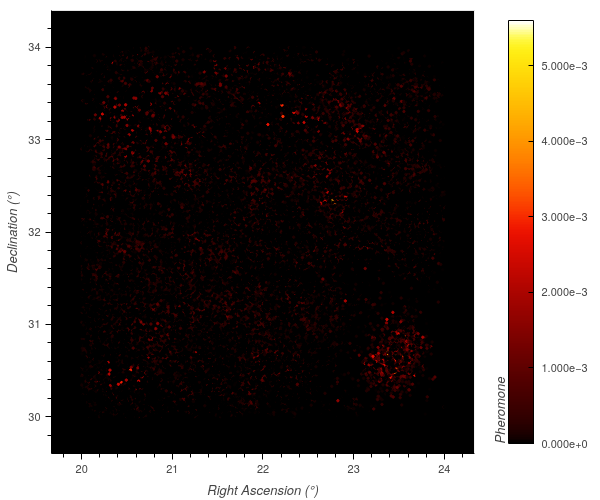
\includegraphics[width=\textwidth]{heatmaps/pheromone-heatmap-a4-20.0-30.0.png}
        \caption{\label{fig:heat-triangulum}A4: Triangulum Gal}
    \end{subfigure}

    \caption{\label{fig:scatterplot-heatmaps-A34} Scatterplots (top) vs. Heat-maps (below) of varying rasters of A3 and A4}
\end{figure}


Table~\ref{tb:Nstars-in-reffig} helps visualize a possible relation between the number of stars present in a raster and the maximum pheromone values present.
\TODO{change values based on pheromone plots}

\begin{table}[H]
    \centering
    \caption{Visualization of the number of stars and maximum pheromone values of Figure~\ref{fig:scatterplot-heatmaps-A12} and Figure~\ref{fig:scatterplot-heatmaps-A34}.}
    \label{tb:Nstars-in-reffig}
    \begin{tabular}{l c c }
        \toprule
        Figure                                                             & $N_{\text{stars}}$ & max pheromone bar \\
        \midrule
        \ref{fig:scatter-ngc4147} A1 NGC 4147                              & 5612               & 3.75              \\
        \ref{fig:scatter-palomar5} A1 Palomar5 + M5                        & 19290              & 1.50              \\
        \ref{fig:scatter-M71-dog-4b4} A2 (4x4)                             & 1391301            & 0.55              \\
        \ref{fig:scatter-M71-dog-2b2} A2 (2x2)                             & 331916             & 0.75              \\
        \ref{fig:scatter-small-magellanic-cloud} A3 Small Magellanic Cloud & 239828             & 0.50              \\
        \ref{fig:scatter-large-magellanic-cloud} A3 Large Magellanic Cloud & 523931             & 1.75              \\
        \ref{fig:scatter-andromeda} A4 Andromeda                           & 21587              & 0.90              \\
        \ref{fig:scatter-triangulum} A4 Triangulum                         & 14568              & 3.25              \\
        \bottomrule
    \end{tabular}
\end{table}


\subsection{Stats on the pheromone distribution \textbf{per area}:}

The Ant Colony algorithm outputs a pheromone value for every star in the data-set. The stars that were not visited by an ant have a pheromone value nearly set to zero and the ones that were visited have a pheromone value somewhere between zero and ??. The pheromone distribution can be seen in Figure \ref{fig:areas-hist-pheromone}
\TODO{rerun pheromone distribution stats plot}

\begin{figure}[H]
    \centering
    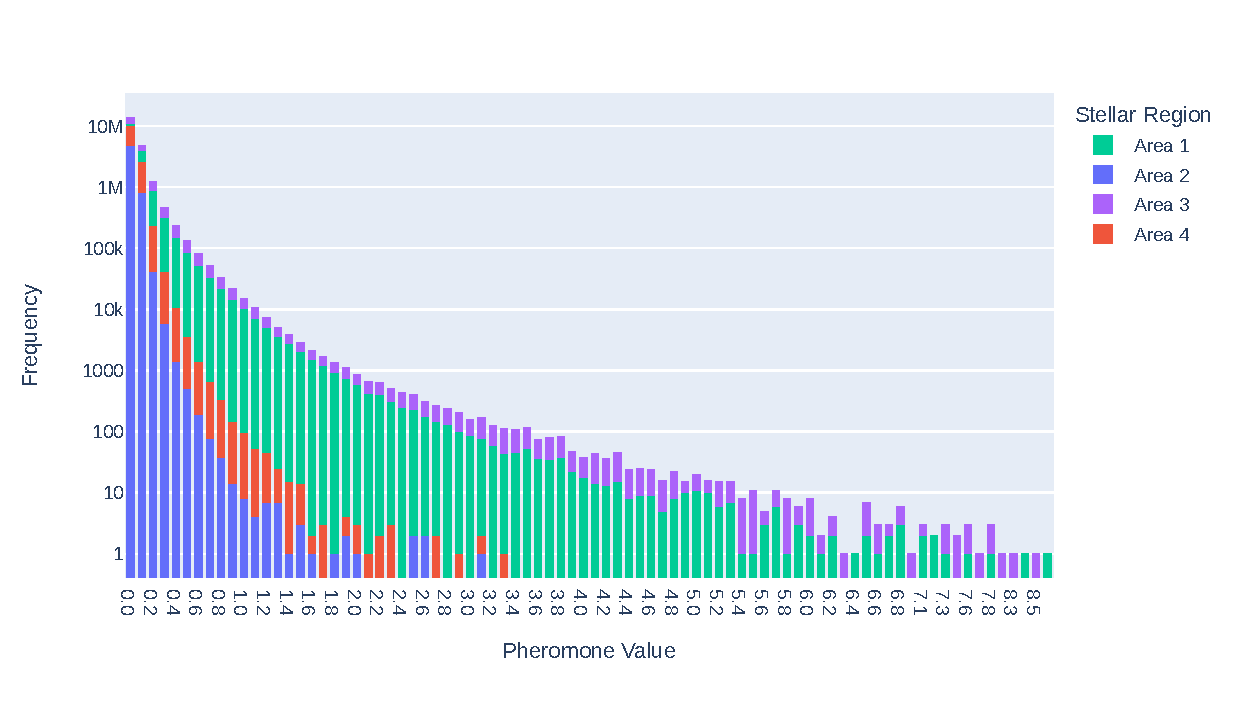
\includegraphics[width=\textwidth]{histograms/pheromone-histogram.pdf}
    \caption{\label{fig:areas-hist-pheromone} Logarithmic Distribution of Pheromone for the Four Areas}
\end{figure}



When looking at Table~\ref{tb:pheromone-mean-areas}, it becomes clear that not only the distribution of A1 and A3, and A2 and A4 are similar but also the mean ($\mu$) pheromone values. The $\mu$ pheromone values of the visited stars in A1 and A3 lie around \num{0.16} and in A2 and A4 they lie around \num{0.04}.

\TODO{rerun this as well}

\begin{table}[H]
    \centering
    \begin{tabular}{l c c c }
        \toprule
        Area     & $\mu$ pheromone value of the visited stars \\
        \midrule
        A1       & 0.1654                                     \\
        A2 (2x2) & 0.0345                                     \\
        A3       & 0.1545                                     \\
        A4       & 0.0515                                     \\
        \bottomrule
    \end{tabular}
    \caption{The mean ($\mu$) pheromone values per area}
    \label{tb:pheromone-mean-areas}
\end{table}


\subsection{Stars Visited per Area}

\TODO{compute the percentage visited per area for A2 (4x4) comment on why it is or is not different}.

The total number of visitations ($N_{\text{visitations}}$) per raster that can happen is determined by the number of ants, steps, and generations; $N_{a} \times N_{s} \times N_{\text{gens}}$ = $N_{\text{visitations}}$ total. With the default values for the ants, steps, and generations $N_{\text{visitations}}$, $30 \times \num{1000} \times 5$, makes \num{150000}. This number is not spread out evenly over all stars as the focus of the algorithm is to have the ants visit the most dense parts of the rasters, which is where the visitations are high and where the ants will hang around. As the number of stars per area and the approximation of stars per raster is of different size and the total possible $N_{\text{visitations}}$ is the stays the same, the number of visited stars and the percentage of stars visited per area is diverse for the different areas.

\TODO{rerun the visited stars and recalculate the percentage}

\begin{table}[H]
    \centering
    \begin{tabular}{l c c c c}
        \toprule
        Area     & Number of Stars & Approximation of Stars per Raster & Visited Stars & Percentage (\%) \\
        \midrule
        A1       & \num{3540521}   & \num{6915}                        & \num{2658150} & 75.1            \\
        A2 (2x2) & \num{5745034}   & \num{164144}                      & \num{871919}  & 15.1            \\
        A3       & \num{4031209}   & \num{14145}                       & \num{1583441} & 39.3            \\
        A4       & \num{7374125}   & \num{61451}                       & \num{2002229} & 27.2            \\
        \bottomrule
    \end{tabular}
    \caption{The percentage of stars visited in the Ant Algorithm, per area}
    \label{tb:visited-stars-percentage}
\end{table}

The average percentage is about 34\%. However, when looking at each area you can see that the percentage visited in A1 is much higher than A2. This is likely explained by the difference in star population density for these areas. The number of stars that reside in A2 is nearly to double the number that reside in A1 while A1 is much larger than A2. Which means there are more stars per raster but the algorithm still is set the same, has a set number of ants, with a set number of steps, and a set number of rounds that it will do. The low percentage is not unexpected and has been tried to be accounted for by having a smaller raster for A2, however, this still led to an average of 15\% of visited stars in A2. A smaller raster means that the algorithm gets run on a smaller set of stars each time, increasing the number of visited stars, however the danger is that when splitting up the stars, one might divide the GC into pieces. It depends on where the dataset is cut on whether this GC division happens.
% area1:(126x62),area2:(13x10),7812/130 = 60.1 times bigger in theory however it is kind of a cone formation and depth does not get accounted in this regard of density. However due to the restrictions of pmra and pmdec, the depth has been limited by elimination so the density is still higher.
% This is an answer to: 'what happens with noise?'


\newpage

\section{\label{sec:data-clustering}Clustering}

\TODO{remake all tables, and rerun the numbers}

The output of the clustering will show the final results of the pipeline. Where it has detected a cluster and what stars belong to this cluster. In Figure \ref{fig:clusterplots-ngc5053-2d} it becomes clear how the pheromone values have an influence on the clustering output. The pheromone values are clearly visible in the right upper corner of the pheromone heat-map, and so is the cluster also found in the same location (right upper corner), as can be easily seen in this 2D cluster plot.


\TODO{It still finds GCs in raster a1-196.0-18.0 but there are 3 of them not 2, so the question is if one still wants to use this. one as an example.}


\begin{figure}[H]
    \centering
    \begin{subfigure}[b]{0.49\textwidth}
        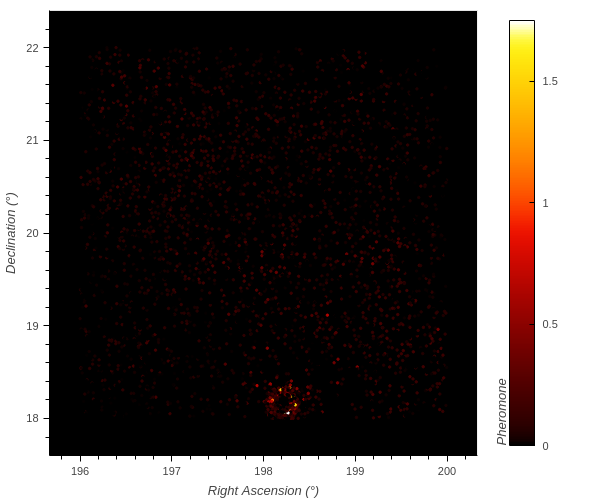
\includegraphics[scale=0.36]{{2d-pipeline-plots/a1-196.0-18.0-heatplot.png}}
        \caption{Pheromone Heat-map}
        \label{fig:ph-3d-1}
    \end{subfigure}
    \begin{subfigure}[b]{0.49\textwidth}
        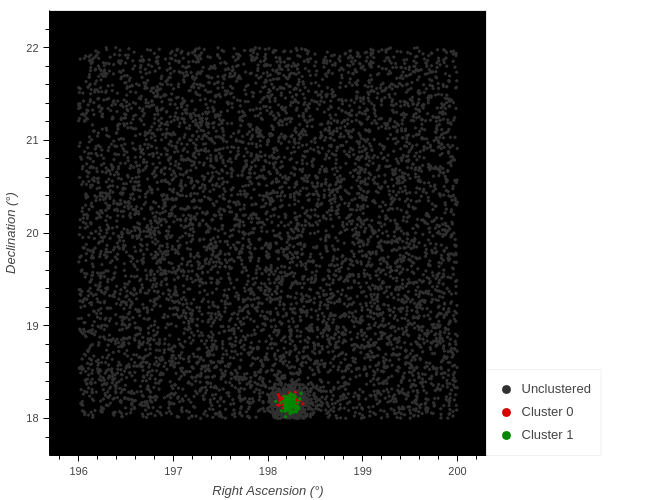
\includegraphics[scale=0.36]{{2d-pipeline-plots/a1-196.0-18.0-clusterplot.png}}
        \caption{Pheromone Heat-map}
        \label{fig:ph-3d-8}
    \end{subfigure}
    \caption{Pheromone Heat-map and Cluster Plot of NGC5025}
    \label{fig:clusterplots-ngc5053-2d}
\end{figure}

The 2D angle which shows the $RA$-$Dec$ side of the clusters location makes it easy to pinpoint its location. However, it cannot give insight on depth and it is unclear about how the stellar sets that were found belong together as cluster formations. To visualize the clustering within a raster, involving information on the depth, 3D plotting is needed.

\begin{figure}[H]
    \centering
    \begin{subfigure}[b]{0.49\textwidth}
        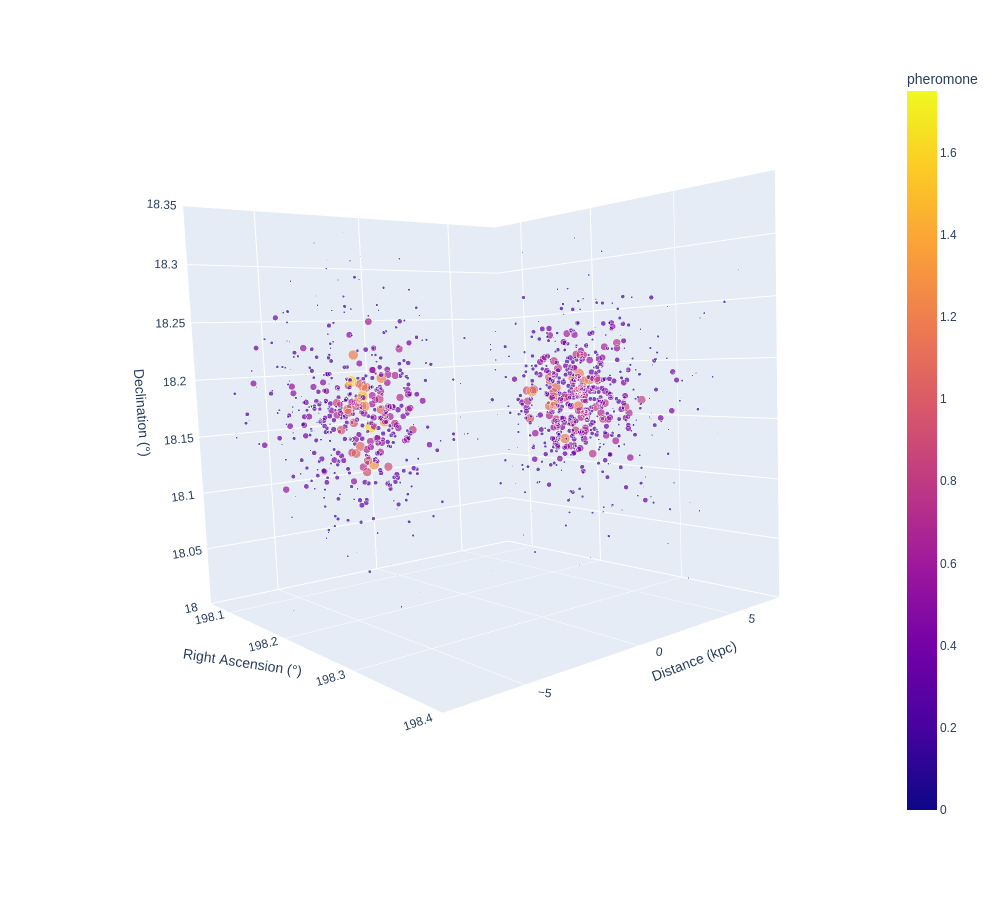
\includegraphics[scale=0.31]{{3d-pipeline-plots/a1-196.0-18.0-heatmap.png}}
        \caption{Pheromone Heat-map}
        \label{fig:ph-3d-18}
    \end{subfigure}
    \begin{subfigure}[b]{0.49\textwidth}
        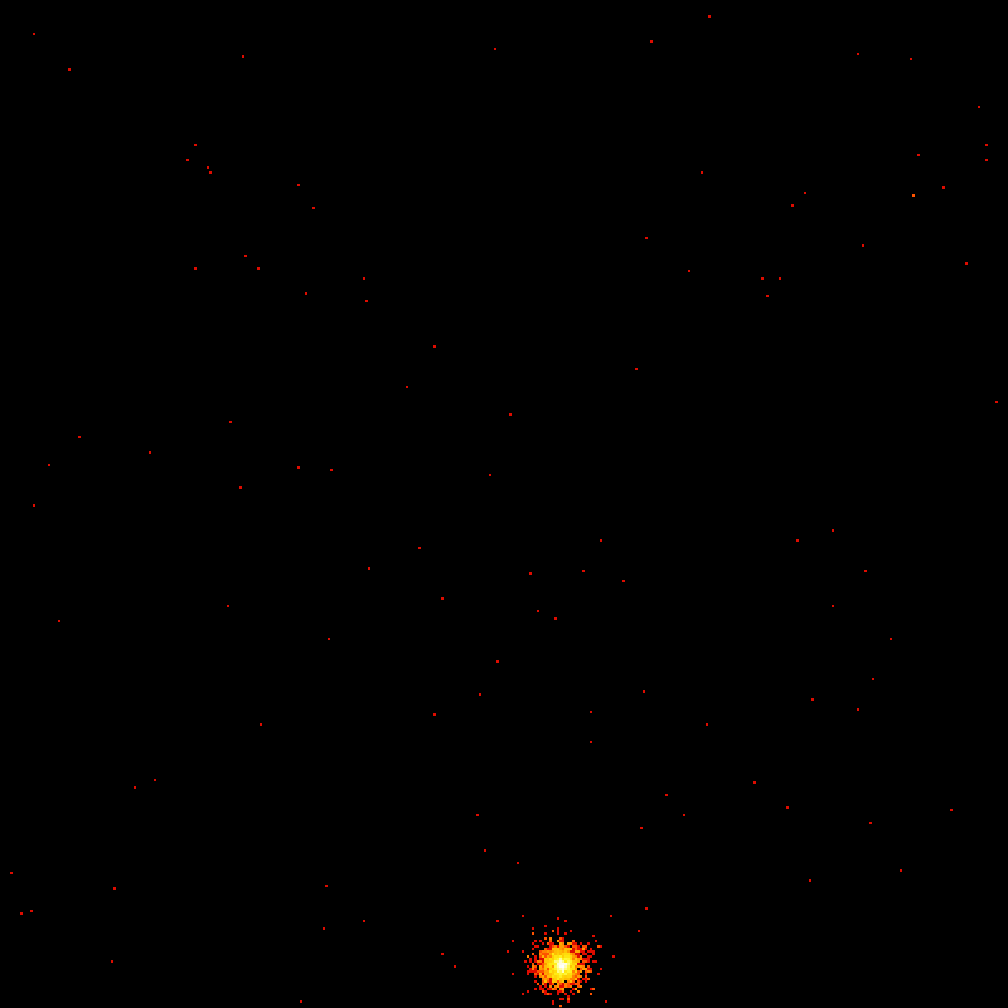
\includegraphics[scale=0.31]{{3d-pipeline-plots/a1-196.0-18.0.png}}
        \caption{3D Cluster Plot}
        \label{fig:cp-3d-18}
    \end{subfigure}
    \caption{3D Plots of NGC 5025}
    \label{fig:3d-NGC5025}
\end{figure}

It specifically gives insight into what is going on in the raster when multiple clusters are found that are overlapping. As the stars with a negative $parallax$ have been kept in the dataset, overlapping clusters might be the same cluster. This assumption could be drawn when the clusters are overlapping and located approximately at each others mirroring $distance$, for example at 5 kpc and -5 kpc, as can be seen in Figure \ref{fig:3d-NGC5025}. To know what GCs might be overlapping you first should check if the clusters are overlapping on the $RA$-$Dec$ side. What this side can indicate is if the clusters are distinct or overlapping clusters. In Figure \ref{fig:distinct-clusters} you can see two clearly distinct clusters: the yellow cluster Cluster 4 and the red cluster Custer 0. In Figure \ref{fig:overlapping-clusters} there are six other clusters hidden behind pink cluster Cluster 6. These could be distinct but will only become clear from investigating the clusters depth locations.

\begin{figure}[H]
    \centering
    \begin{subfigure}[b]{0.49\textwidth}
        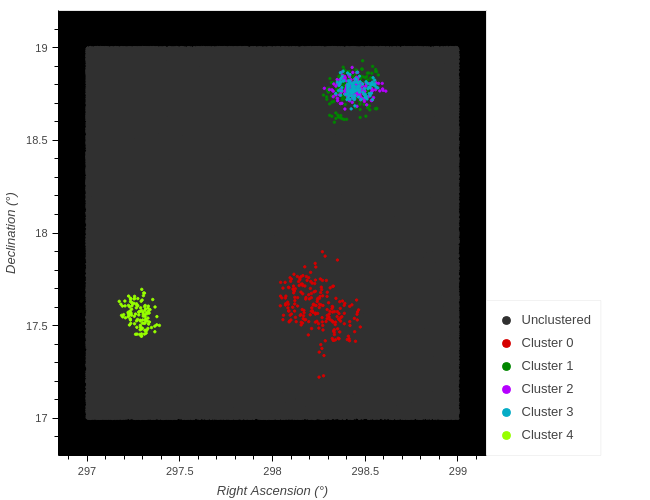
\includegraphics[scale=0.36]{{2d-pipeline-plots/a2-ns-clusterplot.png}}
        \caption{Distinct Clusters example}
        \label{fig:distinct-clusters}
    \end{subfigure}
    \begin{subfigure}[b]{0.49\textwidth}
        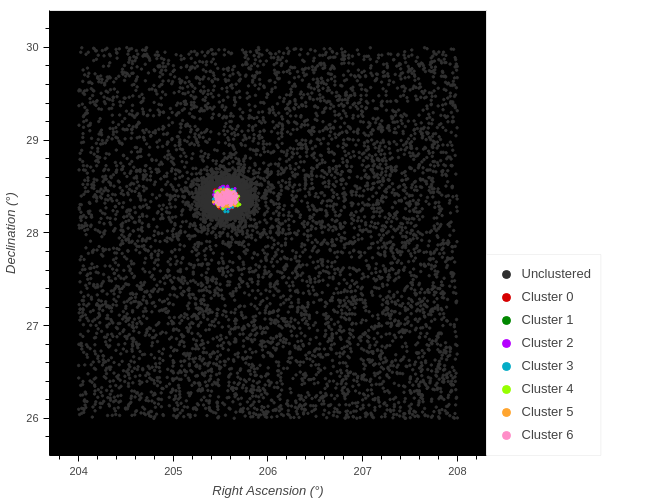
\includegraphics[scale=0.36]{{2d-pipeline-plots/a1-204.0-26.0-clusterplot.png}}
        \caption{Overlapping Clusters example}
        \label{fig:overlapping-clusters}
    \end{subfigure}
    \caption{2D Distinct and Overlapping Clusters}
    \label{fig:2d-distinct-and-overlapping}
\end{figure}


\TODO{For each area an example plot of the 2d pheromone heat-map and the clusters it has found, for area 4 show a plot of what it thinks is a gc. For area 3 show 47 Tucane and the distant cluster which most likely is not found: Arp - Madore 1, maybe NGCs that are really close: 1651 and 1652 (will have to make a table to view which files they are in.) for area 2 show the variations on the GC (\tx{a2_297.0_17.0.bin}) so default (2d and 3d) and the Ns variation on the same raster containing the GC. Also the 3d cluster plot of \tx{a2_307.0_21.0.bin} in default version. Area 1 has the interesting overlapping clusters and otherwise idkn.}



% \begin{figure}[H]
%     \centering
%     \begin{subfigure}[b]{0.49\textwidth}
%         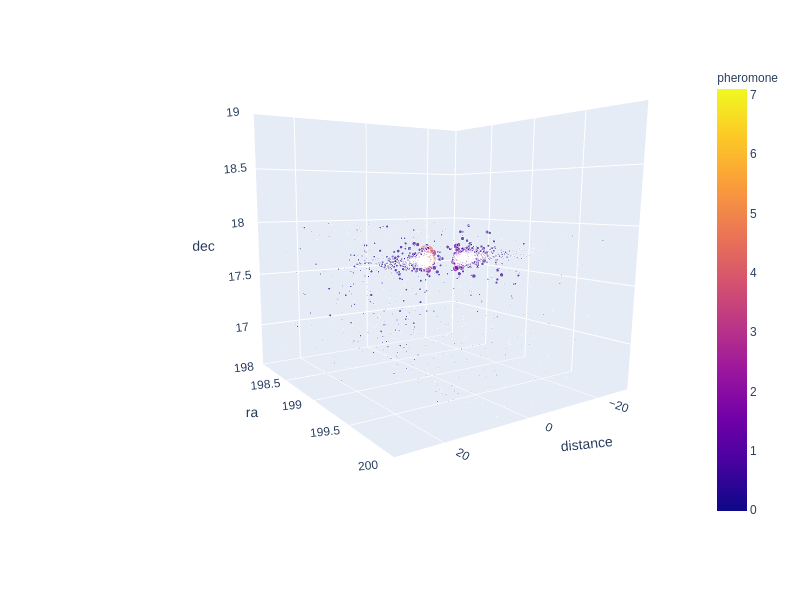
\includegraphics[width=\textwidth]{overlapping-ngcs/3d-overlapping-zoom-ngcs.png}
%         \caption{Pheromone Heat-map}
%         \label{fig:ngcs4}
%     \end{subfigure}
%     \begin{subfigure}[b]{0.49\textwidth}
%         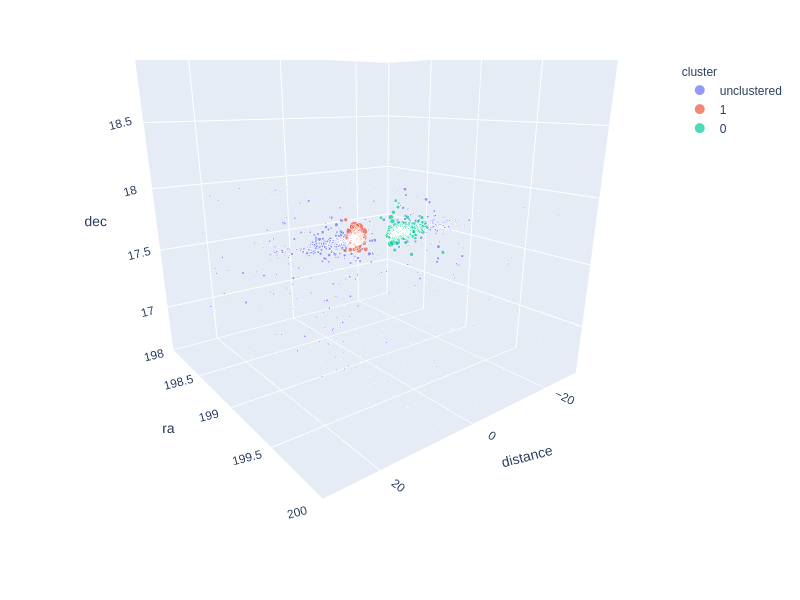
\includegraphics[width=\textwidth]{overlapping-ngcs/ncgs-3d-cluster.png}
%         \caption{Cluster Map}
%         \label{fig:ngcs3}
%     \end{subfigure}
%     \caption{The 3D plots of the overlapping GCs NGC5024 and NGC5053}
%     \label{fig:ngcs}
% \end{figure}


\begin{table}[H]
    \centering
    \begin{tabular}{l c c }
        \toprule
        Area     & Total Clusters Detected & Detected in number of Rasters \\
        \midrule
        A1       & 104                     & 77                            \\
        A2 (2x2) & 2                       & 2                             \\
        A3       & 52                      & 46                            \\
        A4       & 6                       & 5                             \\
        \bottomrule
    \end{tabular}
    \caption{The number of clusters detected in a number of rasters for each area}
    \label{tb:clusters-detected-areas}
\end{table}


\TODO{Make them subfigure tables for each area}
\begin{table}[H]
    \centering
    \caption{What known GCs are getting detected for a threshold of 0.2}
    \label{tb:areas-found-rasters-0.2}
    \begin{tabular}{l c c c c c l c c}
        \toprule
        GC        & Present? & In (?/5) & GC     & Present? & In (?/5) & GC           & Present & In (?/5) \\
        \midrule
        Area 1    &          &          & Area 2 &          &          & Area 3       &         &          \\
        \midrule
        M3        & Present  & (5/5)    & M71    & Present  & (2/5)    & 47 Tucanae   &         &          \\
        M5        & special  & (1/5)    &        &          &          & NGC 121      &         &          \\
        NGC 5024  & Present  & (5/5)    &        &          &          & NGC 1049     & Present & (5/5)    \\
        NGC 4147  & Present  & (5/5)    &        &          &          & NGC 362      &         &          \\
        NGC 5053  & Present  & (4/5)    &        &          &          & NGC 1261     & Present & (5/5)    \\
        NGC 5466  & Present  & (5/5)    &        &          &          & NGC 1629     &         &          \\
        Koposov 1 &          &          &        &          &          & NGC 1644     &         &          \\
        Palomar 3 &          &          &        &          &          & NGC 1651     &         &          \\
        Palomar 4 &          &          &        &          &          & NGC 1652     &         &          \\
        Palomar 5 & special  & (1/5)    &        &          &          & NGC 1696     &         &          \\
        GCI 38    &          &          &        &          &          & NGC 1756     &         &          \\
        Willman 1 &          &          &        &          &          & NGC 1783     & Present & (4/5)    \\
                  &          &          &        &          &          & NGC 1786     &         &          \\
                  &          &          &        &          &          & NGC 1795     &         &          \\
                  &          &          &        &          &          & NGC 1841     & Present & (5/5)    \\
                  &          &          &        &          &          & Arp Madore 1 &         &          \\
        \bottomrule
    \end{tabular}
\end{table}

\begin{figure}[H]
    \centering

    \begin{subfigure}[b]{0.49\textwidth}
        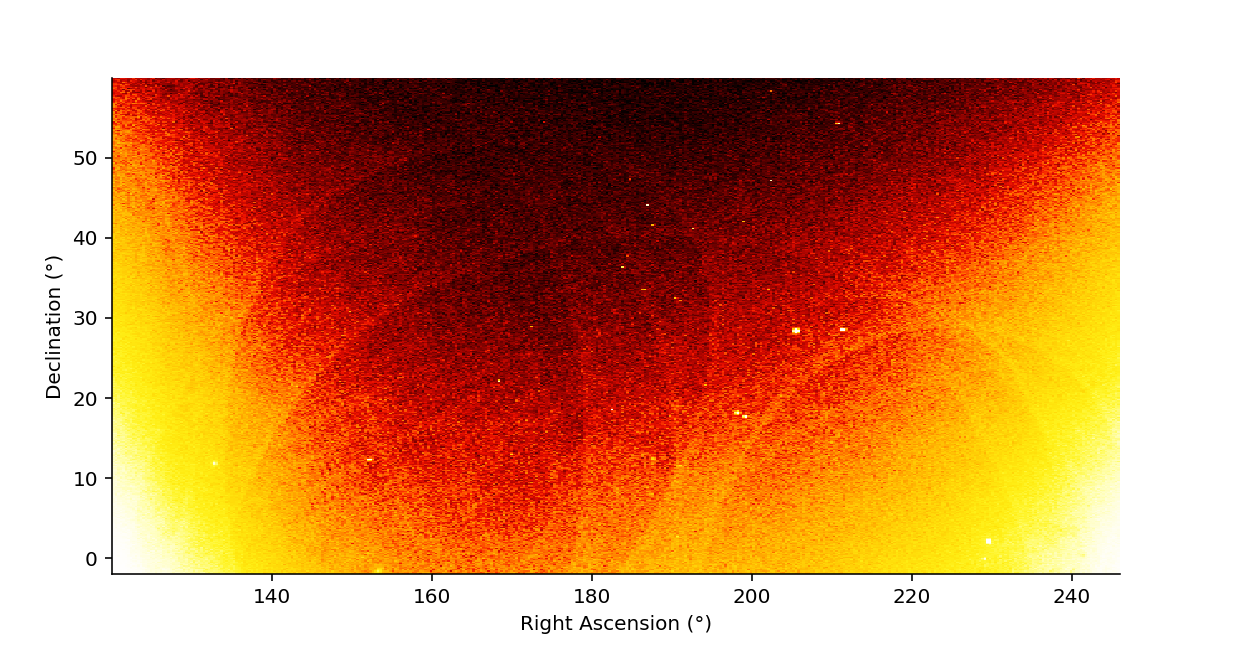
\includegraphics[ height=0.6\textwidth]{scatterplots/area1-scatterplot.png}
        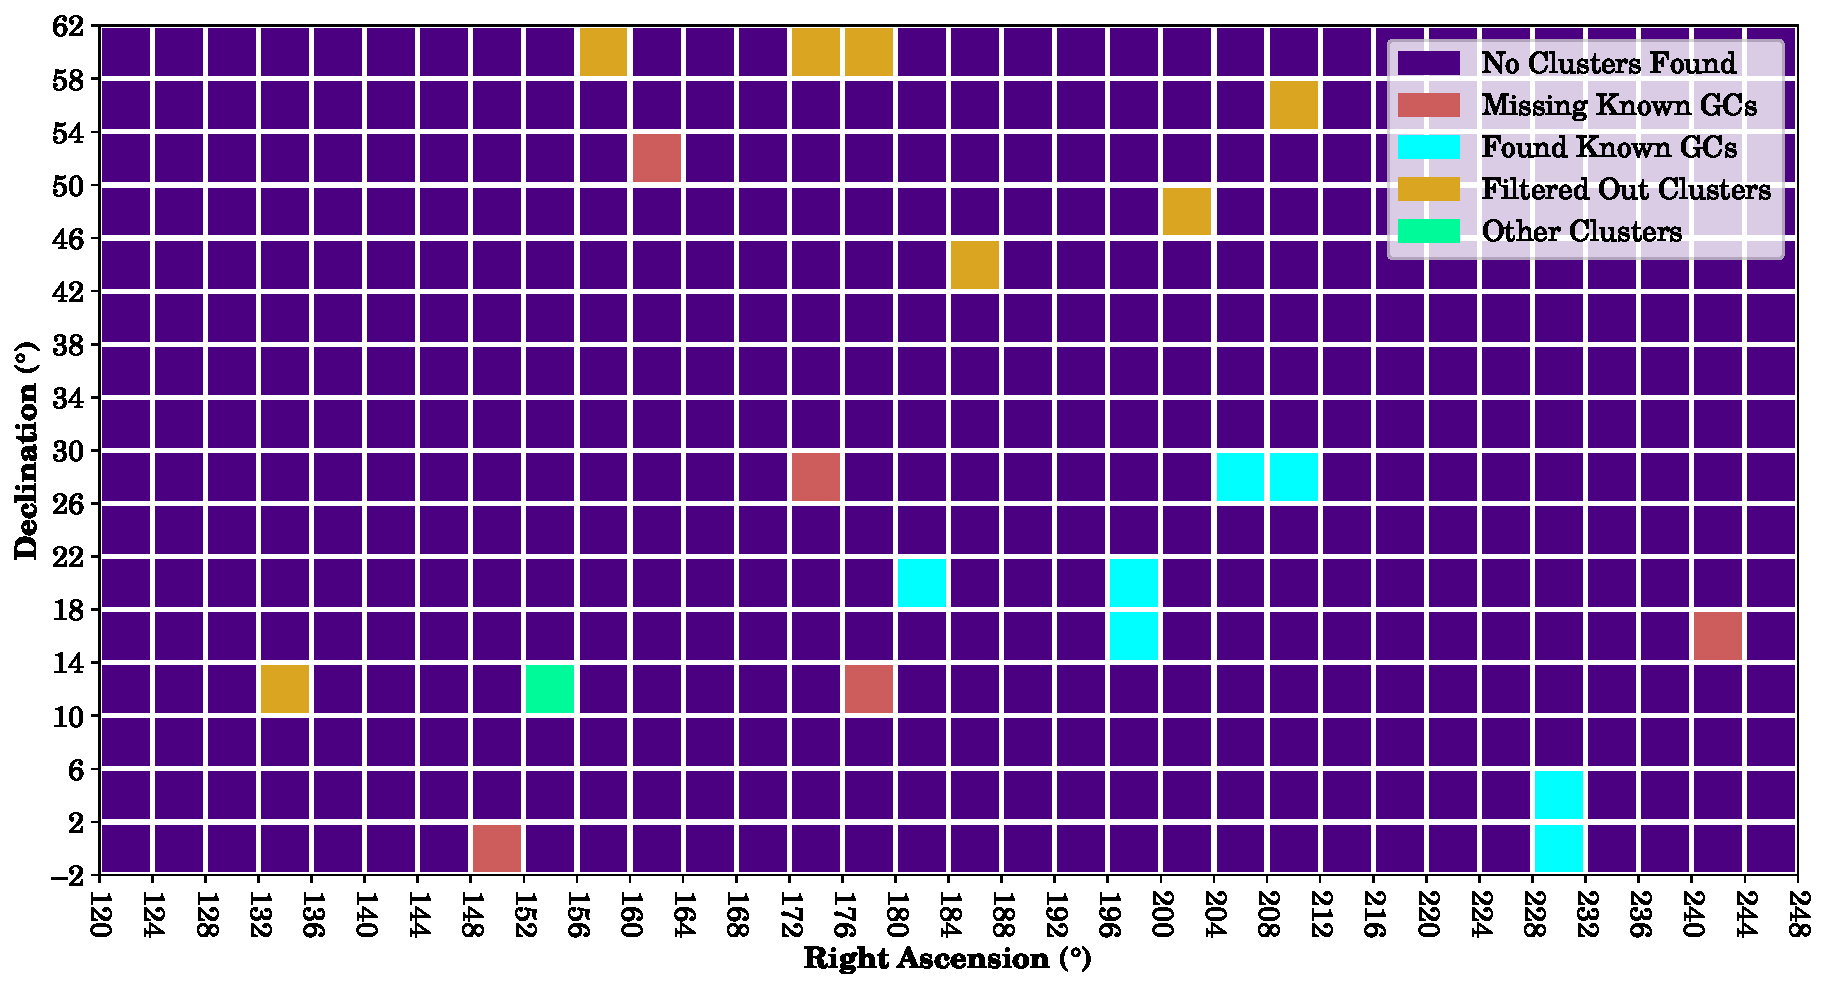
\includegraphics[height=0.6\textwidth]{./figures/rasters/grids/grid-combined-a1.pdf}
        \caption{A1}
        \label{fig:a1-cluster-overview}
    \end{subfigure}
    \begin{subfigure}[b]{0.49\textwidth}
        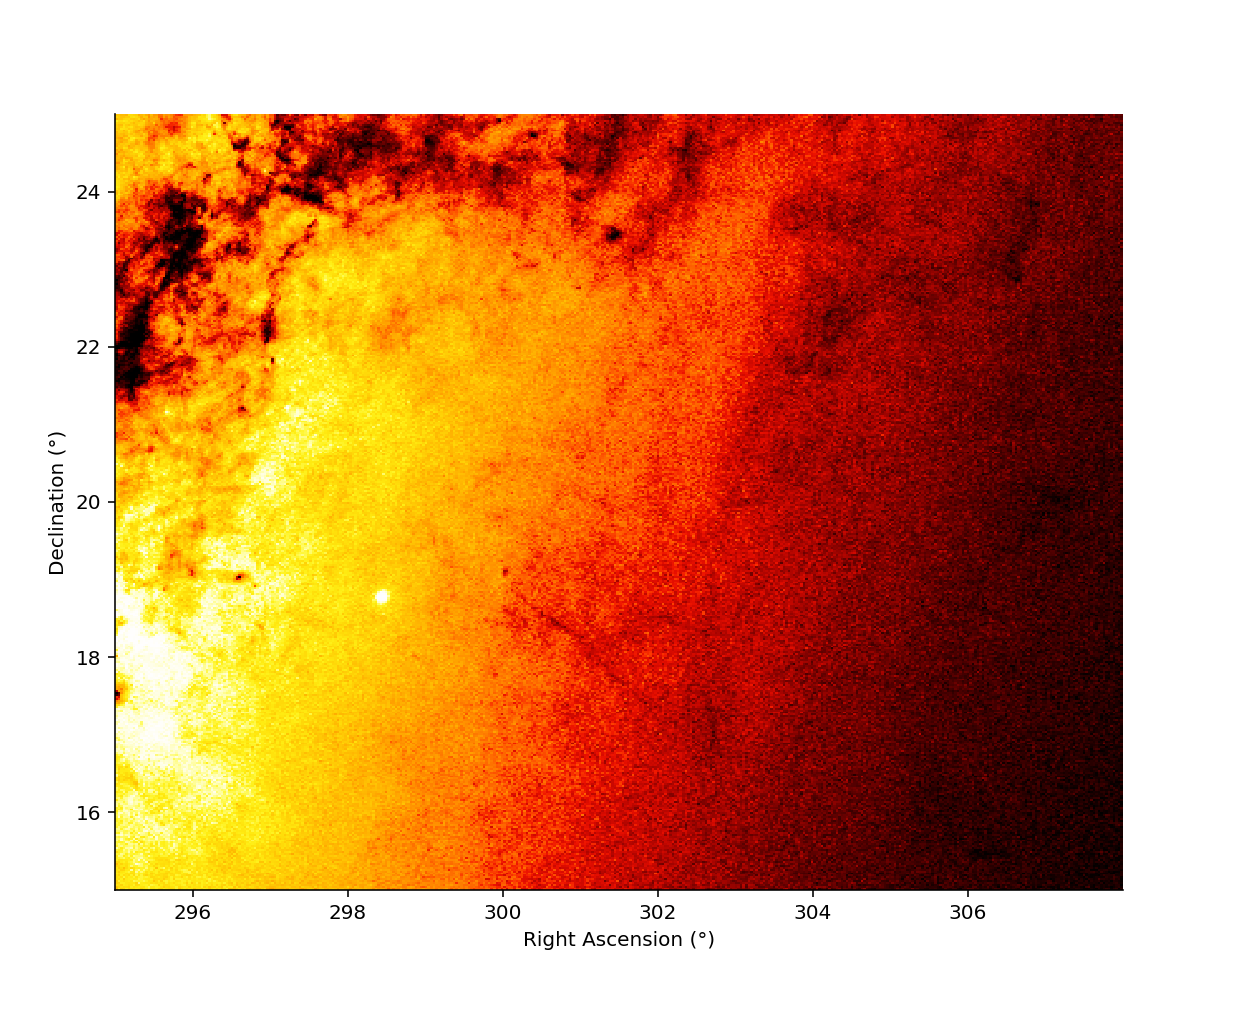
\includegraphics[ height=0.6\textwidth]{scatterplots/area2-scatterplot.png}
        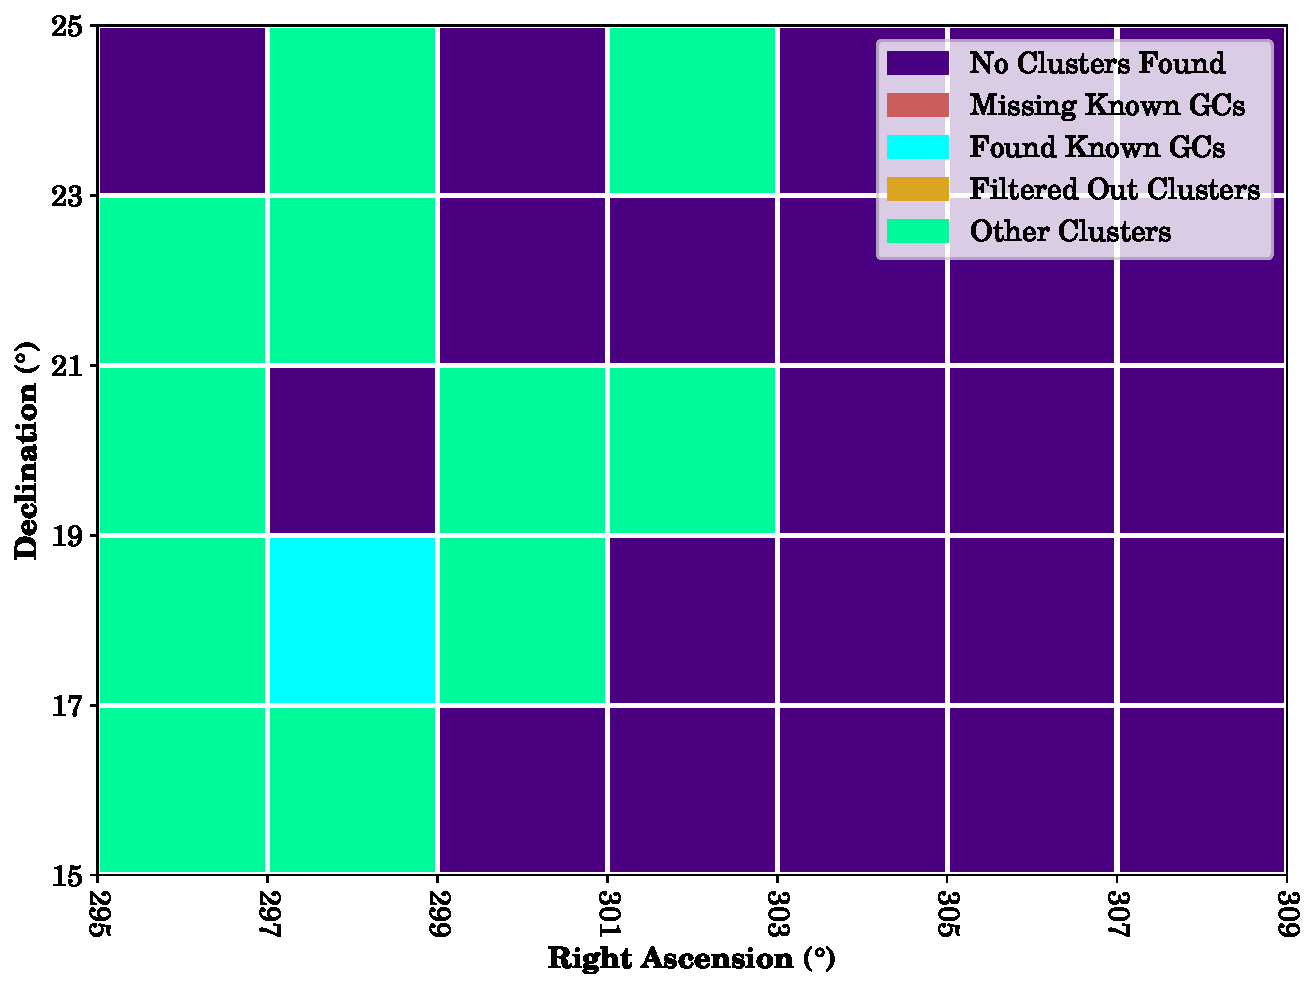
\includegraphics[height=0.6\textwidth]{./figures/rasters/grids/grid-combined-a2.pdf}
        \caption{A2}
        \label{fig:a2-cluster-overview}
    \end{subfigure}

    \begin{subfigure}[b]{0.49\textwidth}
        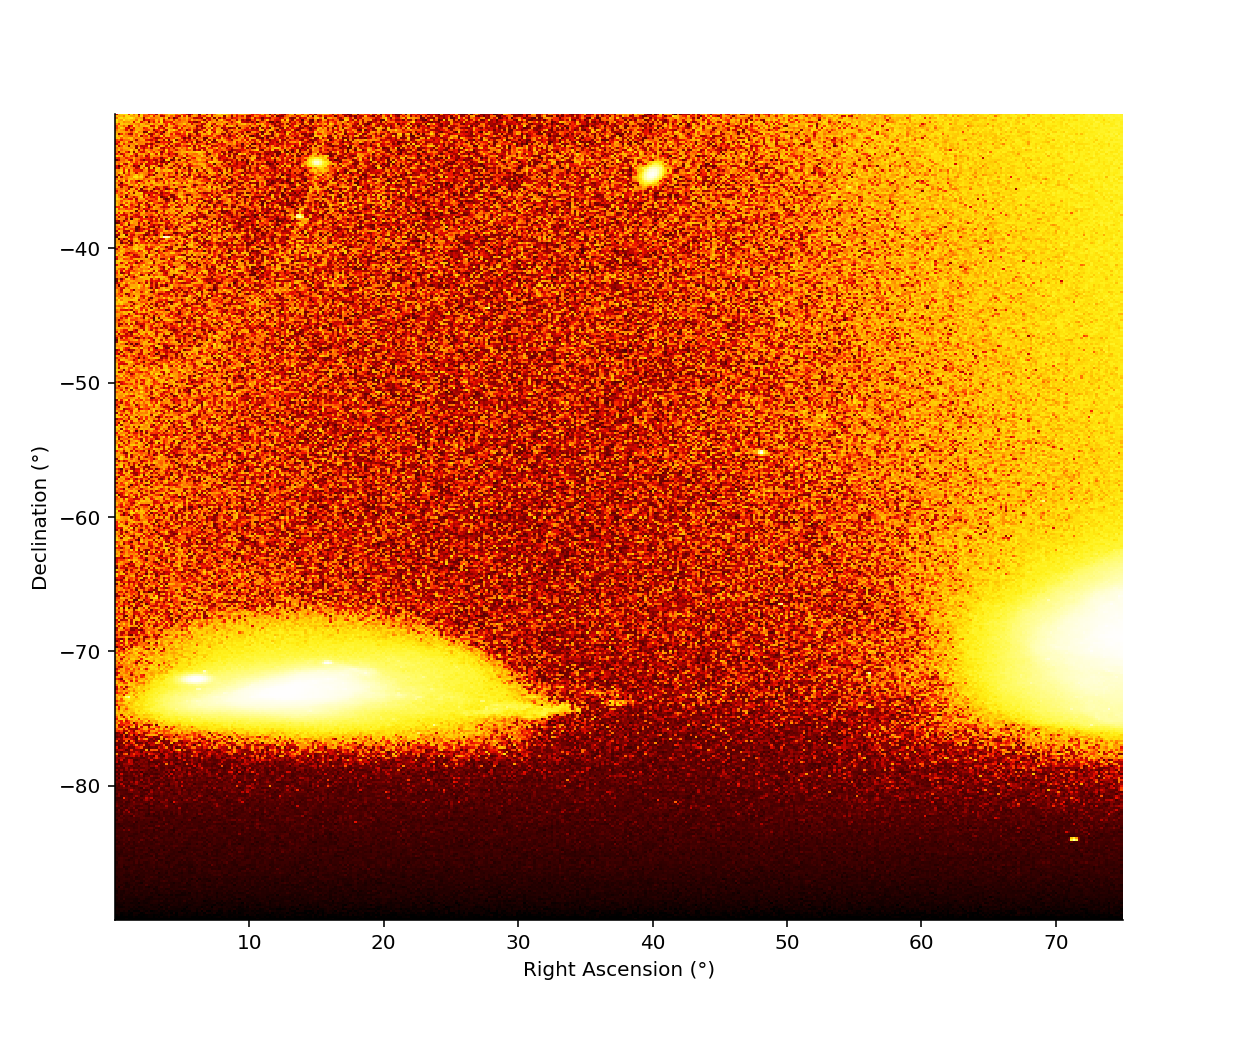
\includegraphics[ height=0.6\textwidth]{scatterplots/area3-scatterplot.png}
        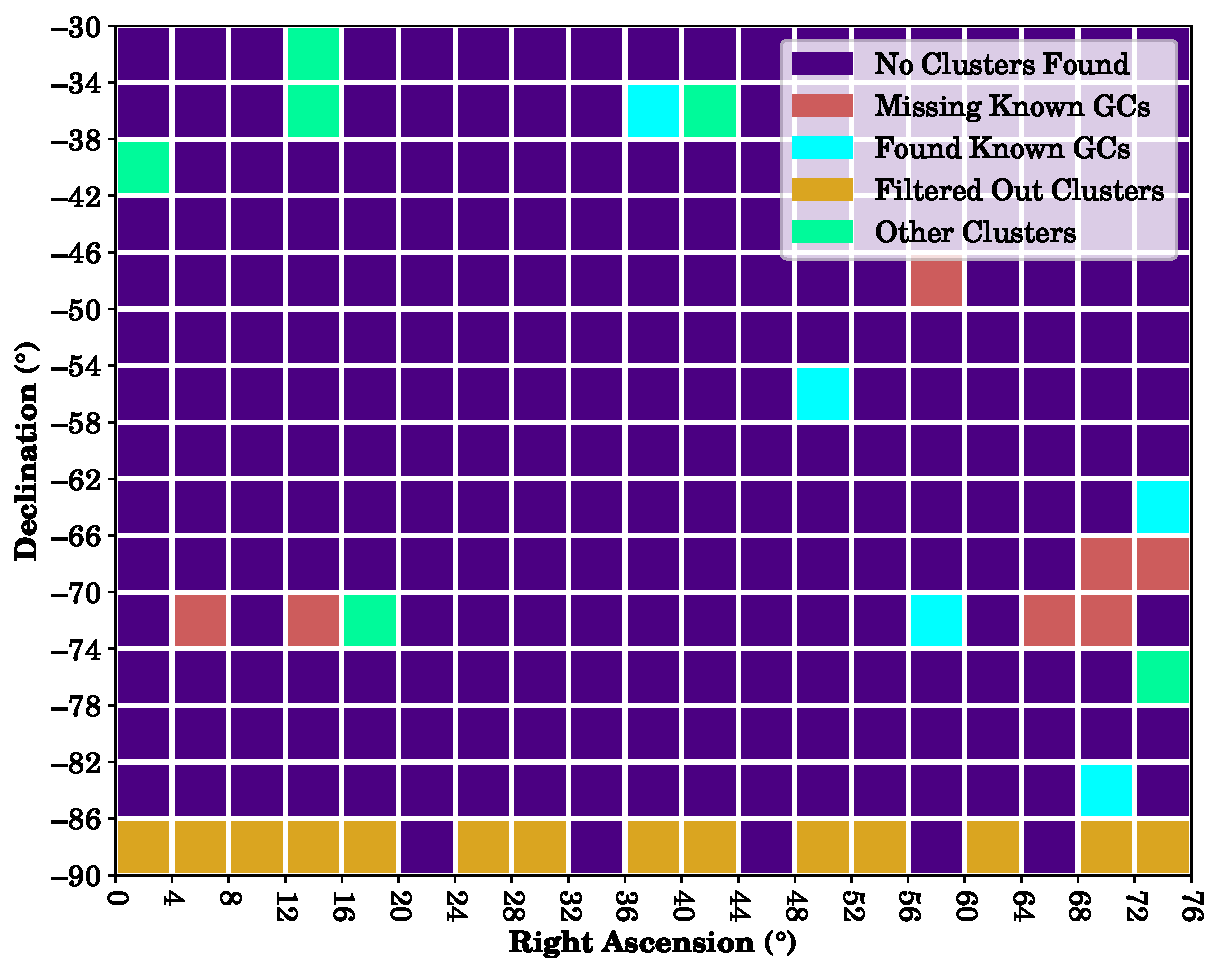
\includegraphics[height=0.6\textwidth]{./figures/rasters/grids/grid-combined-a3.pdf}
        \caption{A3}
        \label{fig:a3-cluster-overview}
    \end{subfigure}
    \begin{subfigure}[b]{0.49\textwidth}
        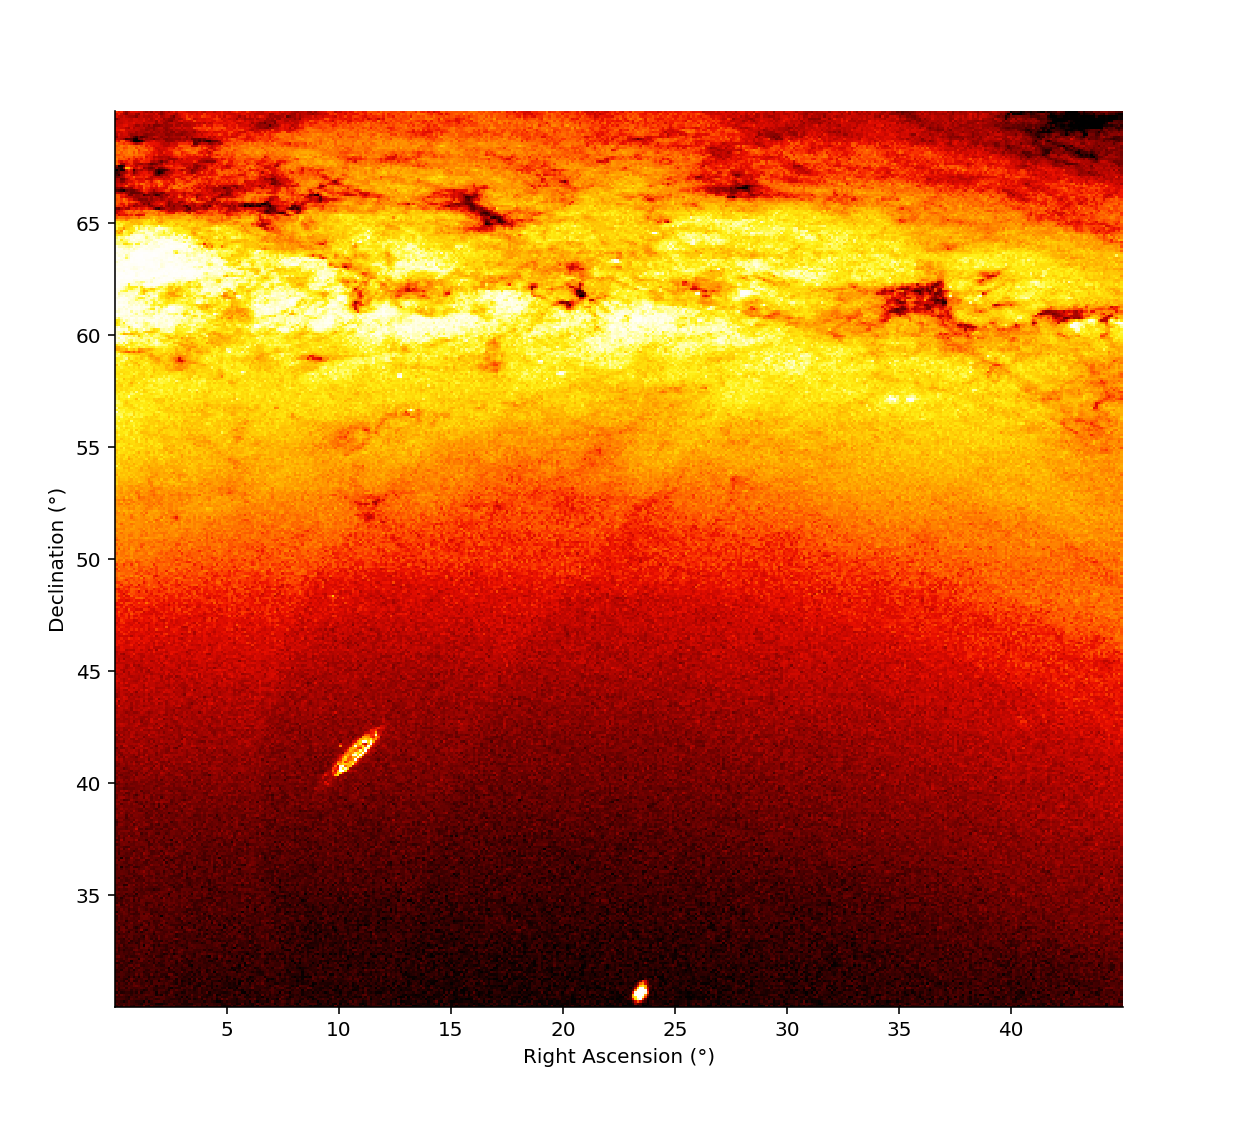
\includegraphics[ height=0.6\textwidth]{scatterplots/area4-scatterplot.png}
        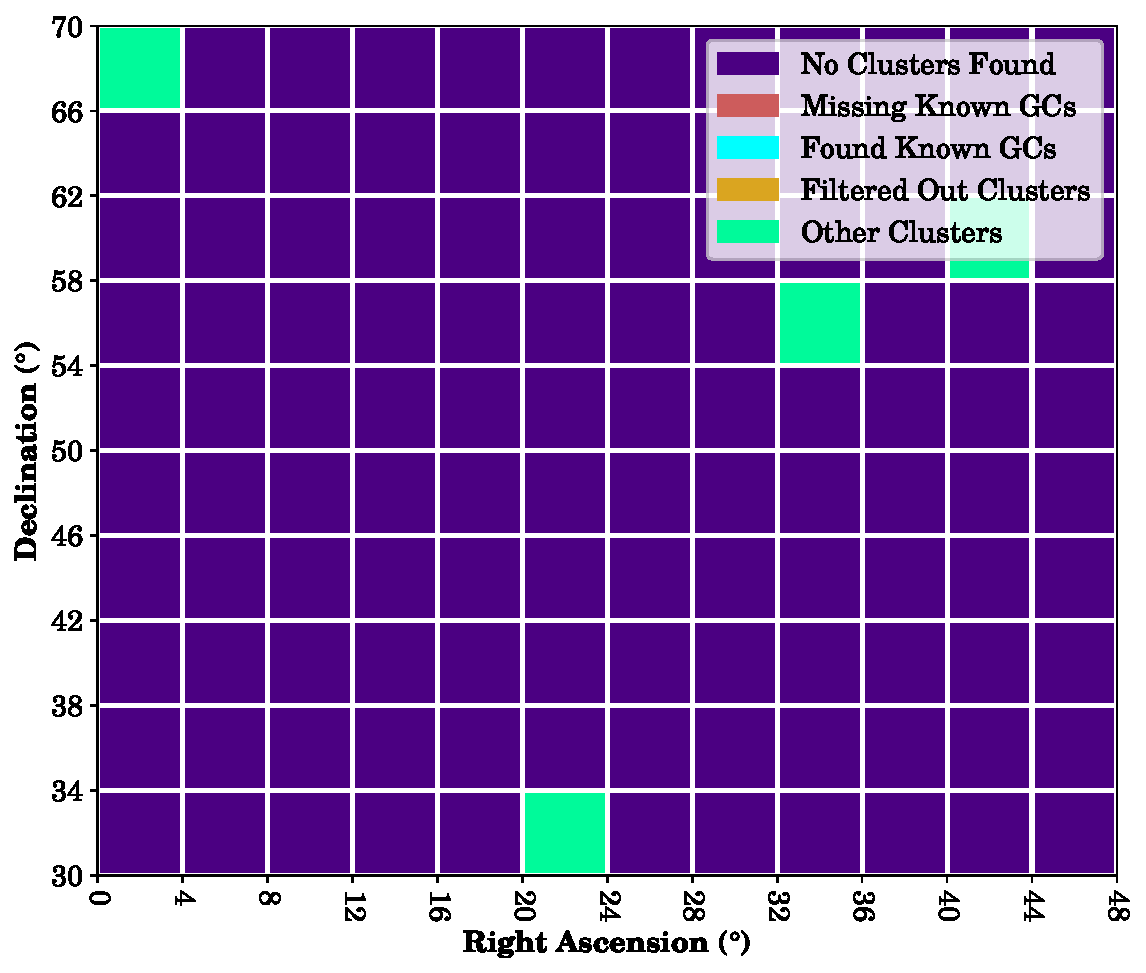
\includegraphics[height=0.6\textwidth]{./figures/rasters/grids/grid-combined-a4.pdf}
        \caption{A4}
        \label{fig:a4-cluster-overview}
    \end{subfigure}

    \caption{Remaining Rasters of Areas After Clustering}
    \label{fig:filtered-cluster-rasters}
\end{figure}

\textbf{Results of Complete Pipeline}

\begin{table}[H]
    \centering
    \begin{tabular}{l c c }
        \toprule
        Area     & Total Clusters Detected & Detected in number of Rasters \\
        \midrule
        A1       & 16                      & 7                             \\
        A2 (2x2) & 1                       & 1                             \\
        A3       & 12                      & 8                             \\
        A4       & 3                       & 2                             \\
        \bottomrule
    \end{tabular}
    \caption{The number of clusters detected in a number of rasters for each area}
    \label{tb:pipeline-clusters-detected}
\end{table}

\begin{table}[H]
    \centering
    \caption{Pipeline Cluster Results}
    \label{tb:pipeline-cluster-results}
    \begin{tabular}[t]{l L{2cm} l l c c}
        \toprule
        \midrule
        \multicolumn{1}{c}{Cluster Type} & \ac{l}{Name}             & \ac{l}{RA (\si{\degree})} & \ac{l}{Dec (\si{\degree})} & \ac{l}{distance (kpc)} & \ac{c}{bounds of distance (kpc)} \\
        \addlinespace[2em]
        \midrule[0.5pt]
        \multicolumn{4}{c}{A1}                                                                                                                                                           \\
        \midrule[0.5pt]
        GC                               & M3                       & \ang{205.55}              & \ang{+28;22;12}            & 6.47                   & 6.07 -- 6.88                     \\
        GC                               & M3                       & \ang{205.56}              & \ang{+28;22;12}            & 4.17                   & 4.01 -- 4.39                     \\
        GC                               & M3                       & \ang{205.55}              & \ang{+28;22;48}            & 4.77                   & 4.41 -- 5.10                     \\
        GC                               & M3                       & \ang{205.56}              & \ang{+28;22;12}            & 5.27                   & 4.99 -- 5.52                     \\
        GC                               & M3                       & \ang{205.57}              & \ang{+28;22;12}            & 7.17                   & 6.93 -- 7.45                     \\
        GC                               & M3                       & \ang{205.55}              & \ang{+28;21;36}            & -4.92                  & -5.09 -- -4.75                   \\
        GC                               & M3                       & \ang{205.56}              & \ang{+28;22;12}            & -4.17                  & -4.33 -- -4.03                   \\
        GC                               & M5                       & \ang{229.63}              & \ang{+2;5;12}              & -4.14                  & -4.32 -- -4.00                   \\
        GC                               & M5                       & \ang{229.64}              & \ang{+2;4;12}              & -5.30                  & -5.53 -- -5.10                   \\
        GC                               & NGC 4147                 & \ang{182.53}              & \ang{+18;42;0}             & 4.76                   & 4.01 -- 5.95                     \\
        GC                               & NGC 5053                 & \ang{199.11}              & \ang{+17;42;0}             & 4.76                   & 4.02 -- 5.79                     \\
        GC                               & NGC 5024                 & \ang{198.23}              & \ang{+18;10;12}            & -5.17                  & -5.73 -- -4.64                   \\
        GC                               & NGC 5024                 & \ang{198.23}              & \ang{+18;9;36}             & 4.55                   & 4.10 -- 5.03                     \\
        GC                               & NGC 5466                 & \ang{211.36}              & \ang{+28;31;48}            & -4.79                  & -5.41 -- -4.18                   \\
        GC                               & NGC 5466                 & \ang{211.37}              & \ang{+28;31;48}            & 4.47                   & 4.07 -- 5.04                     \\
        GC                               & Palomar 5                & \ang{229.62}              & \ang{+1;57;36}             & 4.54                   & 4.01 -- 5.17                     \\
        \addlinespace[2em]
        \midrule[0.5pt]
        \multicolumn{4}{c}{A2}                                                                                                                                                           \\
        \midrule[0.5pt]
        GC                               & M71                      & \ang{298.42}              & \ang{+18;47;24}            & 6.36                   & 6.19 -- 6.53                     \\
        \addlinespace[2em]
        \midrule[0.5pt]
        \multicolumn{4}{c}{A3}                                                                                                                                                           \\
        \midrule[0.5pt]
        unknown                          & 0.0 -78.0                & \ang{3.52}                & \ang{-74;22;48}            & -4.85                  & -5.71 -- -4.01                   \\
        unknown                          & 0.0 -78.0                & \ang{3.58}                & \ang{-74;34;48}            & 4.45                   & 4.01 -- 5.06                     \\
        unknown                          & 0.0 -74.0                & \ang{3.70}                & \ang{-73;30;36}            & 4.40                   & 4.01 -- 4.95                     \\
        Galaxy                           & Southern Pinwheel Galaxy & \ang{13.75}               & \ang{-37;21;0}             & 4.65                   & 4.00 -- 5.79                     \\
        Galaxy                           & Sculptor Dwarf Galaxy    & \ang{15.02}               & \ang{-33;42;36}            & 4.83                   & 4.01 -- 6.06                     \\
        GC                               & NGC 1049                 & \ang{39.81}               & \ang{-34;33;36}            & 4.70                   & 4.00 -- 5.53                     \\
        GC                               & NGC 1049                 & \ang{39.84}               & \ang{-34;33;36}            & -4.41                  & -4.96 -- -4.01                   \\
        Galaxy                           & Fornax Dwarf Galaxy      & \ang{40.16}               & \ang{-34;25;48}            & 4.63                   & 4.02 -- 5.42                     \\
        Galaxy                           & Fornax Dwarf Galaxy      & \ang{40.12}               & \ang{-34;29;24}            & -4.32                  & -4.71 -- -4.02                   \\
        GC                               & NGC 1261                 & \ang{48.08}               & \ang{-55;12;36}            & 4.67                   & 4.01 -- 5.51                     \\
        GC                               & NGC 1261                 & \ang{48.07}               & \ang{-55;13;12}            & -4.49                  & -5.05 -- -4.00                   \\
        GC                               & NGC 1841                 & \ang{71.38}               & \ang{-84;0;36}             & -5.63                  & -7.63 -- -4.06                   \\

        \addlinespace[2em]
        \midrule[0.5pt] \multicolumn{4}{c}{A4}                                                                                                                                           \\
        \midrule[0.5pt]
        Galaxy                           & Triangulum Galaxy        & \ang{23.48}               & \ang{+30;39;0}             & 4.43                   & 4.00 -- 5.04                     \\
        Galaxy                           & Triangulum Galaxy        & \ang{23.45}               & \ang{+30;36;0}             & -4.31                  & -4.72 -- -4.01                   \\
        unknown                          & 16.0 58.0                & \ang{16.22}               & \ang{+60;39;0}             & 4.16                   & 4.01 -- 4.39                     \\

        \midrule
        \bottomrule
    \end{tabular}
\end{table}


The raster of M3 contains seven clusters that overlap at coordinates $ (\ang{205.5}, \ang{28;22;}) $. The mirrored clusters could lie at distances of:
4.17 and -4.17, and 4.77 and -4.92.
The raster of M5 contains two clusters that both lie at a negative distance of -4.14 and -5.30 kpc.

Except for the raster of the known GCs M3 and M5, all overlapping clusters are in pairs that are at opposite parallaxes, one negative and one positive,that almost are at opposite distance values form zero.

If all distances would be assumed as positive the distance of the found clusters lies between: 4.00 and 7.63 kpc.

Koposov 1 has a distance of 48.3 kpc, palomar 4 a distance of 109 kpc, GCI 38 a distance of 74.7 kpc, NGC 121 a distance of 61 kpc, ngc 362 8.5 kpc,  NGC 1783 49 kpc, arp madore 1 123.3 kpc.

47 Tucanae with a distance of 4.5 kpc has not been found, the cause however, is likely that this GC lies in or near the Magellanic clouds so through the density the pipeline has trouble spotting it.



\begin{longtable}{l c c c c c c}
    \caption{Area 1: all found clusters in all rounds} \label{tb:results-raw-a1}                                                      \\

    \toprule
    Type         & Name                              & RA (°)       & Dec (°)             & Distance & Bounds Distance  & Experiments \\
    \midrule
    OC           & Golden-Eye Cluster                & \ang{132.85} & \ang{+11;48;7.41}   & 0.8772   & 0.6950 -- 1.0252 & 1-5         \\ % a1_132.0_10.0.cluster.json
    Dwarf Galaxy & Regulus Dwarf Galaxy              & \ang{152.12} & \ang{+12;18;3.25}   & 0.5577   & 0.1894 -- 1.0089 & 1-5         \\ % run-01 a1_152.0_10.0.cluster.json
    Galaxy       & ?(NGC 3288, NGC 3286)             & \ang{158.86} & \ang{+58;20;16.71}  & 0.6057   & 0.3240 -- 0.8711 & 4           \\ % run-04 a1_156.0_58.0.cluster.json
    Galaxy       & ?(NGC 3770, NGC 3795)             & \ang{174.06} & \ang{+59;12;18.36}  & 0.6306   & 0.3385 -- 0.9751 & 2           \\ % run-02 a1_172.0_58.0.cluster.json
    Galaxy       & ?(PGC 36655, NGC 3838, PGC 36373) & \ang{176.51} & \ang{+58;31;39.37}  & 0.5514   & 0.2723 -- 0.8349 & 1           \\ % run-01 a1_176.0_58.0.cluster.json
    GC           & NGC 4147                          & \ang{182.53} & \ang{+18;32;29.50}  & 0.6482   & 0.2049 -- 1.1459 & 1-5         \\ % run-01 a1_180.0_18.0.cluster.json
    Galaxy       & The Box Galaxy                    & \ang{187.05} & \ang{+44;7;14.98}   & 0.4573   & 0.0999 -- 0.8306 & 1-5         \\ % run-01 a1_184.0_42.0.cluster.json
    GC           & NGC 5053                          & \ang{199.11} & \ang{+17;42;0.84}   & 0.6204   & 0.4264 -- 0.7178 & 0-4         \\ % run-01 a1_196.0_14.0.cluster.json
    GC           & NGC 5024                          & \ang{198.23} & \ang{+18;10;10.68}" & 0.5641   & 0.3867 -- 0.7514 & 1-5         \\ % run-01 a1_196.0_18.0.cluster.json
    GC           & NGC 5024                          & \ang{198.23} & \ang{+18;9;44.51}"  & 0.8146   & 0.7206 -- 0.9050 & 1-3         \\ % run-01 a1_196.0_18.0.cluster.json
    Galaxy       & Whirlpool Galaxy                  & \ang{202.46} & \ang{+47;11;20.97}" & 0.5249   & 0.1928 -- 0.8233 & 1-3,5       \\ % run-01 a1_200.0_46.0.cluster.json
    GC           & M3                                & \ang{205.54} & \ang{+28;22;12.63}" & 0.2633   & 0.1525 -- 0.3683 & 1,2,4,5     \\ % run-01 a1_204.0_26.0.cluster.json
    GC           & M3                                & \ang{205.55} & \ang{+28;22;16.21}" & 0.4425   & 0.3113 -- 0.5646 & 1-5         \\ % run-01 a1_204.0_26.0.cluster.json
    GC           & M3                                & \ang{205.55} & \ang{+28;22;17.10}" & 0.6266   & 0.5496 -- 0.7136 & 1-4         \\ % run-01 a1_204.0_26.0.cluster.json
    GC           & M3                                & \ang{205.55} & \ang{+28;22;52.99}" & 0.8001   & 0.6585 -- 0.9357 & 2-5         \\ % run-02 a1_204.0_26.0.cluster.json
    GC           & M3                                & \ang{205.57} & \ang{+28;22;42.33}" & 1.3605   & 1.2787 -- 1.4545 & 1,5         \\ % run-01 a1_204.0_26.0.cluster.json
    GC           & NGC 5466                          & \ang{211.36} & \ang{+28;31;59.63}" & 0.7967   & 0.4383 -- 1.1424 & 1-5         \\ % run-01 a1_208.0_26.0.cluster.json
    GC           & NGC 5466                          & \ang{211.36} & \ang{+28;31;48.32}" & 1.3195   & 1.1555 -- 1.4880 & 2-5         \\ % run-02 a1_208.0_26.0.cluster.json
    Galaxy       & Pinwheel Galaxy                   & \ang{210.79} & \ang{+54;21;33.69}" & 0.6562   & 0.3226 -- 0.9375 & 1-5         \\ % run-01 a1_208.0_54.0.cluster.json
    GC           & Palomar 5                         & \ang{229.61} & \ang{+1;57;47.14}"  & 0.6944   & 0.5445 -- 0.8387 & 3           \\ % run-03 a1_228.0_-2.0.cluster.json
    GC           & M5                                & \ang{229.64} & \ang{+2;3;26.66}"   & 1.1115   & 1.0410 -- 1.1732 & 2           \\ % run-02 a1_228.0_2.0.cluster.json
    \bottomrule
\end{longtable}

\begin{table}[H]
    \centering
    \caption{Area 2: all found clusters in all rounds}
    \label{tb:results-raw-a2}
    \begin{tabular}{l c c c c c c }
        \toprule
        Type                                           & Name                & RA (°)       & Dec (°)            & Distance & Bounds Distance  & Experiments \\
        \midrule
        nothing                                        & N.A.                & \ang{296.05} & \ang{+15;19;35.71} & 1.2065   & 1.1459 -- 1.2763 & 4           \\ % run-04 a2_295.0_15.0.cluster.json
        nothing                                        & N.A.                & \ang{295.84} & \ang{+17;28;32.99} & 1.6137   & 1.5096 -- 1.6891 & 3,5         \\ % run-03 a2_295.0_17.0.cluster.json
        dark nebula                                    & ?(LDN 757)          & \ang{295.83} & \ang{+19;9;17.96}  & 1.1144   & 1.0348 -- 1.2180 & 1,3         \\ % run-01 a2_295.0_19.0.cluster.json
        cluster associated with nebulosity, HII region & NGC 6823, NGC 6820, & \ang{296.10} & \ang{+22;27;18.78} & 1.3472   & 1.2446 -- 1.4457 & 3,4         \\ % run-03 a2_295.0_21.0.cluster.json
        nothing                                        & N.A.                & \ang{297.72} & \ang{+15;37;39.26} & 1.4043   & 1.2646 -- 1.5093 & 4           \\ % run-04 a2_297.0_15.0.cluster.json
        GC                                             & M71                 & \ang{298.45} & \ang{+18;46;27.04} & 1.2352   & 1.1693 -- 1.3201 & 1,4         \\ % run-01 a2_297.0_17.0.cluster.json
        nothing                                        & N.A.                & \ang{297.91} & \ang{+21;21;28.57} & 0.9844   & 0.8782 -- 1.0694 & 2,5         \\ % run-02 a2_297.0_21.0.cluster.json
        dark nebula                                    & ?(LDN 791, LDN 789) & \ang{297.17} & \ang{+23;52;8.87}  & 0.7136   & 0.6206 -- 0.7925 & 1           \\ % run-01 a2_297.0_23.0.cluster.json
        nothing                                        & N.A.                & \ang{299.78} & \ang{+18;26;40.78} & 2.3262   & 2.2185 -- 2.4382 & 3,5         \\ % run-03 a2_299.0_17.0.cluster.json
        nothing                                        & N.A.                & \ang{299.71} & \ang{+20;7;38.33}  & 0.3923   & 0.2265 -- 0.5016 & 4           \\ % run-04 a2_299.0_19.0.cluster.json
        nothing                                        & N.A.                & \ang{301.47} & \ang{+19;52;50.56} & 1.3887   & 1.1915 -- 1.5530 & 3           \\ % run-03 a2_301.0_19.0.cluster.json
        molecular cloud                                & ?(LDN 797)          & \ang{302.15} & \ang{+23;29;50.72} & 1.6371   & 1.5381 -- 1.7693 & 5           \\ % run-05 a2_301.0_23.0.cluster.json
        \bottomrule
    \end{tabular}
\end{table}

\begin{longtable}{l c c c c c c}
    \caption{Area 3: all found clusters in all rounds} \label{tb:results-raw-a3}                                                          \\
    \toprule
    Type                & Name                             & RA (°)      & Dec (°)            & Distance & Bounds Distance  & Experiments \\
    \midrule
    Galaxy              & Spring of Pearls                 & \ang{3.78}  & \ang{-39;12;55.81} & 0.4756   & 0.1269 -- 0.8823 & 1-5         \\ % run-01 a3_0.0_-42.0.cluster.json
    galaxy              & ?(PGC 3533, PGC 993)             & \ang{1.37}  & \ang{-86;17;26.62} & 0.7774   & 0.3376 -- 1.3014 & 1-5         \\ % run-01 a3_0.0_-90.0.cluster.json
    Dwarf Galaxy        & Sculptor Dwarf Galaxy            & \ang{15.03} & \ang{-33;43;18.83} & 0.8924   & 0.4708 -- 1.3466 & 1-5         \\ % run-01 a3_12.0_-34.0.cluster.json
    Galaxy              & Southern Pinwheel Galaxy         & \ang{13.72} & \ang{-37;39;30.95} & 0.6512   & 0.1856 -- 1.2625 & 1-5         \\ % run-01 a3_12.0_-38.0.cluster.json
    Galaxy              & ?(PGC 993)                       & \ang{13.58} & \ang{-87;4;29.60}  & 0.8176   & 0.4237 -- 1.1877 & 1-5         \\ % run-01 a3_12.0_-90.0.cluster.json
    Galaxy              & ?(PGC 3533, PGC 216800)          & \ang{12.56} & \ang{-86;31;6.35}  & 0.8366   & 0.3013 -- 1.3887 & 1-3,5       \\ % run-01 a3_12.0_-90.0.cluster.json
    Galaxy              & ?(PGC 3533, PGC 216800)          & \ang{12.45} & \ang{-86;28;57.56} & 0.8124   & 0.3602 -- 1.2840 & 4           \\ % run-04 a3_12.0_-90.0.cluster.json
    OC                  & NGC 419                          & \ang{17.07} & \ang{-72;52;56.38} & 0.3771   & 0.2468 -- 0.5102 & 2           \\ % run-02 a3_16.0_-74.0.cluster.json
    Galaxy              & ?(PGC 3533, PGC 216800)          & \ang{17.19} & \ang{-86;27;15.29} & 0.7938   & 0.3299 -- 1.3106 & 1-5         \\ % run-01 a3_16.0_-90.0.cluster.json
    nothing             & N.A.                             & \ang{25.77} & \ang{-86;27;20.33} & 0.8725   & 0.3818 -- 1.4201 & 1-5         \\ % run-01 a3_24.0_-90.0.cluster.json
    nothing             & N.A.                             & \ang{28.41} & \ang{-86;23;35.26} & 0.7535   & 0.3731 -- 1.2219 & 1-5         \\ % run-01 a3_28.0_-90.0.cluster.json
    GC                  & NGC 1049                         & \ang{39.88} & \ang{-34;32;40.44} & 0.6276   & 0.3582 -- 0.9042 & 1-5         \\ % run-01 a3_36.0_-38.0.cluster.json
    cluster of Galaxies & Abell 3037                       & \ang{36.95} & \ang{-86;20;27.39} & 0.8600   & 0.4662 -- 1.2993 & 1-4         \\ % run-01 a3_36.0_-90.0.cluster.json
    Galaxy              & ?(PGC 3533, PGC 216800, PGC 993) & \ang{7.21}  & \ang{-86;32;40.25} & 1.0201   & 0.4665 -- 1.5901 & 2-5         \\ % run-02 a3_4.0_-90.0.cluster.json
    Galaxy              & Fornax Dwarf Galaxy              & \ang{40.08} & \ang{-34;28;20.89} & 0.4724   & 0.2345 -- 0.7284 & 1-5         \\ % run-01 a3_40.0_-38.0.cluster.json
    Galaxy              & Fornax Dwarf Galaxy              & \ang{40.08} & \ang{-34;31;27.76} & 0.8496   & 0.6855 -- 1.0361 & 1-5         \\ % run-01 a3_40.0_-38.0.cluster.json
    Galaxy              & N.A.                             & \ang{41.01} & \ang{-86;36;28.26} & 0.8114   & 0.2398 -- 1.4314 & 1-5         \\ % run-01 a3_40.0_-90.0.cluster.json
    GC                  & NGC 1261                         & \ang{48.07} & \ang{-55;12;55.14} & 0.3730   & 0.2103 -- 0.5364 & 1-5         \\ % run-01 a3_48.0_-58.0.cluster.json
    GC                  & NGC 1261                         & \ang{48.07} & \ang{-55;12;22.52} & 0.8275   & 0.6819 -- 0.9690 & 1-5         \\ % run-01 a3_48.0_-58.0.cluster.json
    nothing             & N.A.                             & \ang{50.75} & \ang{-86;25;27.67} & 0.9027   & 0.5176 -- 1.3287 & 1-5         \\ % run-01 a3_48.0_-90.0.cluster.json
    nothing             & N.A.                             & \ang{53.58} & \ang{-86;21;39.43} & 0.7970   & 0.4293 -- 1.2832 & 2-4         \\ % run-02 a3_52.0_-90.0.cluster.json
    GC                  & NGC 1466                         & \ang{56.14} & \ang{-71;39;40.54} & 0.8338   & 0.3572 -- 1.4311 & 1,3-5       \\ % run-01 a3_56.0_-74.0.cluster.json
    Galaxy              & PGC 269561                       & \ang{61.90} & \ang{-86;18;41.33} & 0.8083   & 0.3929 -- 1.2762 & 1,3-5       \\ % run-01 a3_60.0_-90.0.cluster.json
    cluster of Galaxies & ?(Abell 3333, Abell s480)        & \ang{62.75} & \ang{-86;32;21.73} & 0.7865   & 0.3562 -- 1.2664 & 1,3-5       \\ % run-01 a3_60.0_-90.0.cluster.json
    GC                  & NGC 1841                         & \ang{71.37} & \ang{-84;0;26.52}  & 1.1711   & 0.3788 -- 2.1652 & 1-5         \\ % run-01 a3_68.0_-86.0.cluster.json
    cluster of Galaxies & ?(Abell 3333)                    & \ang{69.40} & \ang{-86;39;36.30} & 0.9044   & 0.3603 -- 1.6042 & 1-5         \\ % run-01 a3_68.0_-90.0.cluster.json
    cluster of Galaxies & Abell 3333                       & \ang{71.48} & \ang{-86;24;13.19} & 0.7808   & 0.3693 -- 1.2422 & 4,5         \\ % run-04 a3_68.0_-90.0.cluster.json
    GC                  & NGC 1783                         & \ang{74.79} & \ang{-65;58;47.65} & 0.4486   & 0.2693 -- 0.6486 & 1-3,5       \\ % run-01 a3_72.0_-66.0.cluster.json
    GC                  & NGC 1783                         & \ang{74.79} & \ang{-65;58;29.80} & 0.9935   & 0.8451 -- 1.1443 & 2,3,5       \\ % run-02 a3_72.0_-66.0.cluster.json
    OC                  & NGC 1777                         & \ang{73.95} & \ang{-74;16;45.35} & 0.8789   & 0.3516 -- 1.4390 & 1-5         \\ % run-01 a3_72.0_-78.0.cluster.json
    cluster of Galaxies & Abell 3333                       & \ang{73.30} & \ang{-86;37;41.98} & 0.9417   & 0.3151 -- 1.7330 & 1-5         \\ % run-01 a3_72.0_-90.0.cluster.json
    Galaxy              & ?(PGC 3533, PGC 216800)          & \ang{8.62}  & \ang{-86;30;21.61} & 0.7904   & 0.4090 -- 1.1971 & 1-5         \\ % run-01 a3_8.0_-90.0.cluster.json
    \bottomrule
\end{longtable}

\begin{table}[H]
    \centering
    \caption{Area 4: all clusters found in all rounds}
    \label{tb:results-raw-a4}
    \begin{tabular}{l c c c c c c}
        \toprule
        Type       & Name                             & RA (°)      & Dec (°)             & Distance & Bounds Distance  & Experiments \\
        \midrule
        HII region & NGC 7822                         & \ang{0.55}  & \ang{+67;25;22.17}  & 1.0516   & 0.8419 -- 1.2411 & 1-4         \\ % run-01 a4_0.0_66.0.cluster.json
        Galaxy     & Triangulum                       & \ang{23.47} & \ang{+30;36;37.92}  & 0.5641   & 0.3722 -- 0.7355 & 1-5         \\ % run-01 a4_20.0_30.0.cluster.json
        OC         & Double cluster (NGC 869, NGC884) & \ang{35.52} & \ang{+57;8;26.09}   & 2.3437   & 2.2362 -- 2.4466 & 03          \\ % run-03 a4_32.0_54.0.cluster.json
        OC         & NGC 1027                         & \ang{40.69} & \ang{+61;35;27.79}" & 1.1289   & 1.0360 -- 1.2195 & 04          \\ % run-04 a4_40.0_58.0.cluster.json
        \bottomrule
    \end{tabular}
\end{table}

\begin{itemize}
    \item N.A.: stands for Not Applicable
    \item HII region: emission nebula where young star formation is taking place. So a young star forming complex.
    \item The Double Cluster (also known as Caldwell 14) consists of the open clusters NGC 869 and NGC 884 (often designated h Persei and χ (chi) Persei, respectively), which are close together in the constellation Perseus. Both visible with the naked eye, NGC 869 and NGC 884 lie at a distance of about 7,500 light years in the Perseus Arm of the Milky Way galaxy.
    \item \TODO{NGC 1466: Is a GC I missed in the listing, but it was found}
\end{itemize}
